\chapter[Si(Li) tracker flight components validation]{Si(Li) tracker flight components \\validation} \label{ch2}

This Chapter provides a detailed description of the test setup and the test procedures followed to validated the flight items that will be used for the final assembly of the Si(Li) tracker of the GAPS detector. For each of the flight items, a report has been produced in order to detail all the most important parameters with their measured values. Every component has also been uniquely numbered following a specific alphanumeric pattern that can briefly sum up its most relevant characteristics, allowing it to be immediately recognised during the assembly process. This Chapter also provides a deep explanation of the results obtained during the testing activity on all the flight components.

\par
Tests were conducted in order to verify the integrity and proper functioning of the following items:

\begin{enumerate}
    %\bfseries
    \itemsep0em 
    \item Front-End Board (FEB).
    \item Dummy-1 front-end board.
    \item Flex-rigid board.
    \item Connector for termination.
    \item Front-end board shield.
\end{enumerate}

\par
The following Sections are structured as follows: First, the test setup used to verify the correct functioning of the component will be described and a description of the tests performed will be provided, then the results of the tests performed will be reported. 


\hyperref[figFlowChart]{Figure \ref{figFlowChart}} shows the flowchart associated with the testing and validation process of all flight items.

\begin{figure}[h!]
    \centering
    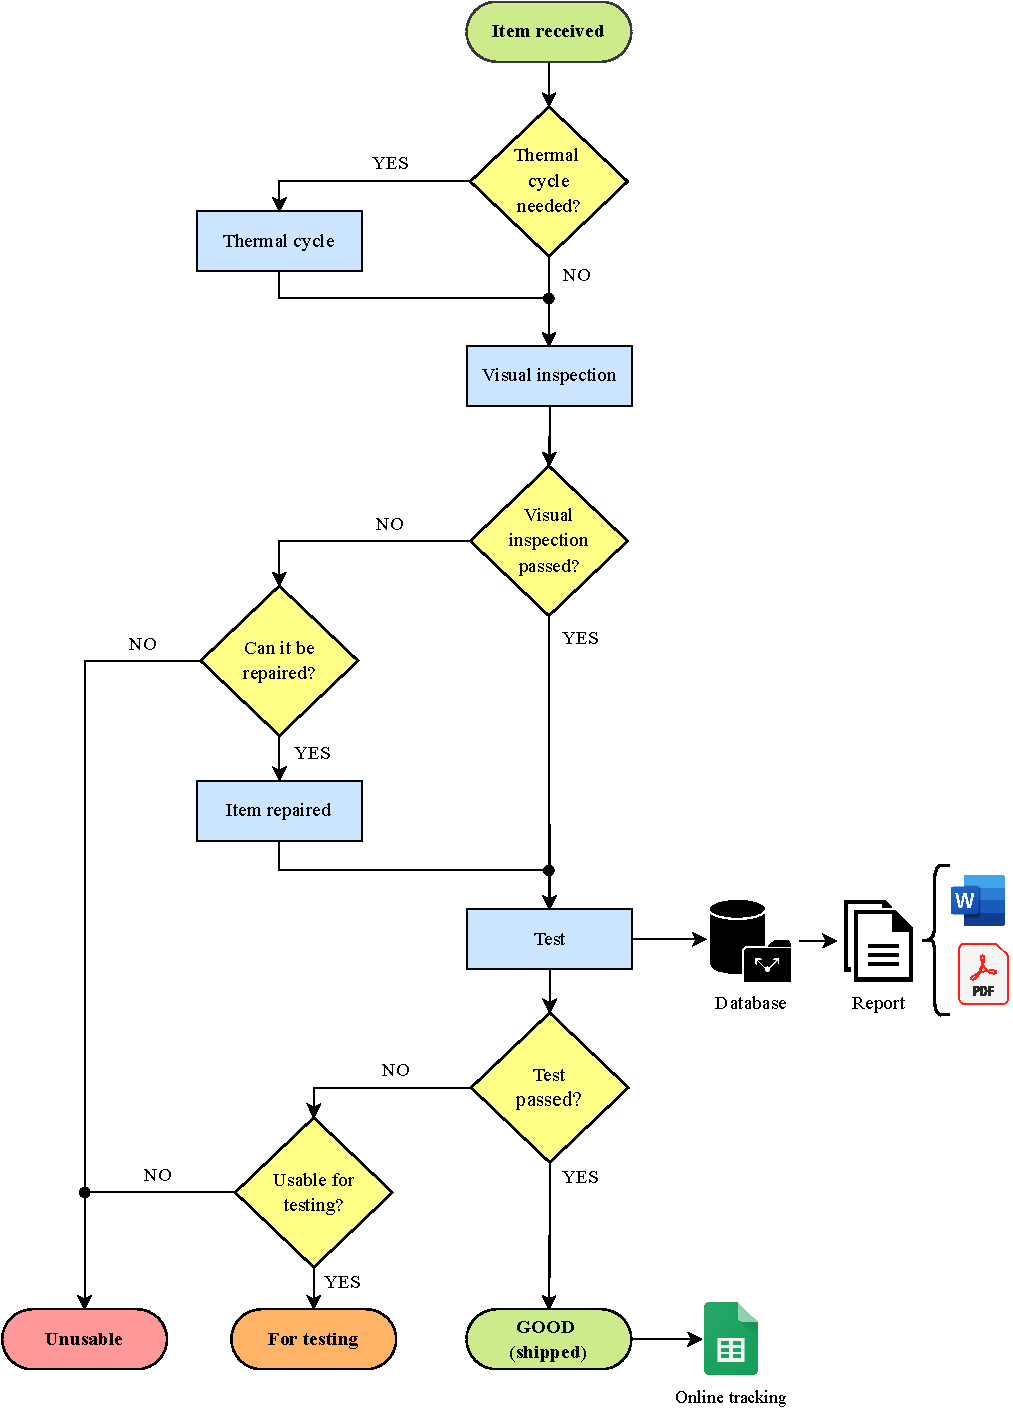
\includegraphics[width=0.8\textwidth]{Images/chap2/flight_item_validation_procedure.drawio.pdf}
    \caption{Flight item validation procedure flowchart.}
    \label{figFlowChart}
\end{figure}

At the end of the test procedure, test results are saved in a database and an item report is generated. Depending on the outcome of the tests performed, the item is classified as:

\begin{itemize}
    \item \textbf{GOOD}, meaning it passed all tests and can be used for tracker assembly.
    \item \textbf{USABLE for testing activity only}, if the component had a defect that was repaired.
    \item \textbf{UNUSABLE}, in case the component had a defect that could not be repaired.
\end{itemize}

\par
\noindent
The items classified as \textbf{GOOD} have been shipped to \textit{Columbia University} to be integrated into the experiment assembly process.


%-------------------------------------------------------------------------------
%   front-end board
%-------------------------------------------------------------------------------

\section{Front-End Board (FEB)} \label{sec21}

\par
The Front-End Board (FEB) that houses the SLIDER32 ASIC is shown in \mbox{\hyperref[figFEBimage]{Figure \ref{figFEBimage}}}. The board was designed in a cross-like shape to make room for the four Si(Li) detectors which will be wire-bonded to the ASIC through the smooth vertical tracks running in the central section of the FEB.

\begin{figure}[ht]
    \centering
    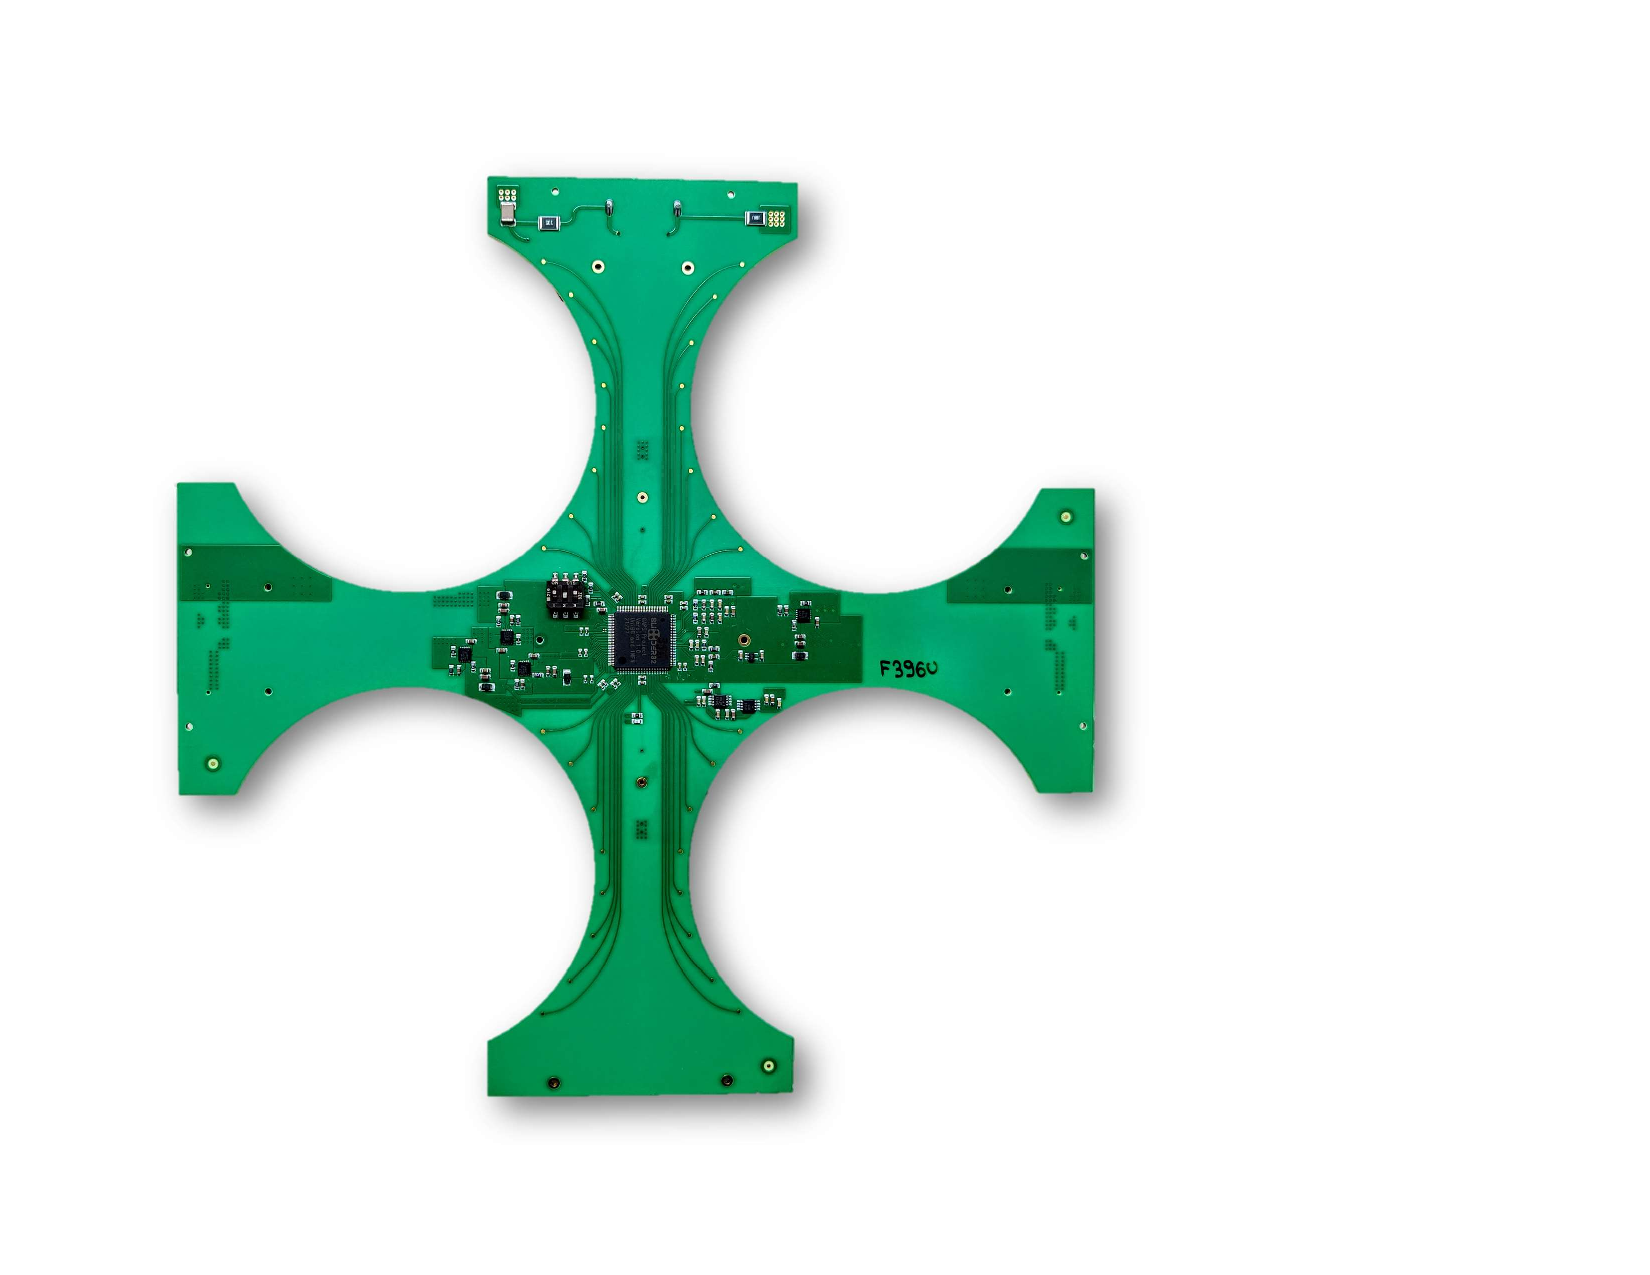
\includegraphics[width=0.7\textwidth]{Images/chap2/FEB_immagine.pdf}
    \caption{SLIDER32 front-end board No. \texttt{F396U} (US production).}
    \label{figFEBimage}
\end{figure}

\par
Each FEB houses the components necessary for the operation of the ASIC and Si(Li) sensors, including the power supplies, divided into High Voltage Power Supply (HVPS) required for the four detectors, and Low Voltage Power Supply (LVPS) necessary for the polarisation of the ASIC and its internal components. Each FEB is also equipped with a current reference for the Charge Sensitive Amplifier (CSA) input transistor, pull-up and pull-down resistors used in the transmission of the control signals, a 3-bit switch to set the address of the FEB, a 16-bit DAC for calibration and a temperature sensor. Within the tracker of the GAPS experiment, the FEBs will be connected to each other via an ERNI connector and a flex-rigid board, later described in \hyperref[flexrigids]{Section \ref{flexrigids}}. Each FEB is equipped with a male (model \texttt{254877}) and female (model \texttt{354178}) ERNI high-speed micro connectors, one used to connect the front-end board to the previous one and the other used to connect it to the following FEB.

\par

\par
The test of the front-end boards has been performed at ambient temperature and was aimed at verifying the proper functioning of the board and at looking for damages to the board or improperly soldered components, including the aforementioned ERNI connectors. The test has been performed in a twofold way:

\begin{itemize}
    \itemsep0em 
    \item By measuring the DC operating point of the ASIC with a Fluke 79 III digital multimeter and a Keysight N6705C DC Power analyser (with N6762A and N6733B modules installed);
    \item By running a purposely developed automated validation test controlled by a terasIC OpenVino Toolkit based on an ALTERA Cyclone V Field Programmable Gate Array (FPGA) board. This procedure performs several types of tests, which are summarised in the following list:
    
    \begin{enumerate}
        %\bfseries
        \itemsep0em 
        \item Noise (ENC).
        \item Pedestal.
        \item Self trigger.
        \item Threshold scan.
        \item Channel input-output characteristic.
        \item Waveform scan.
    \end{enumerate}
\end{itemize}

\par
A detailed representation of the setup used for the tests is reported in \hyperref[figFEBtest1]{Figure \ref{figFEBtest1}} and in \hyperref[figFEBtest2]{Figure \ref{figFEBtest2}}. At first, the setup depicted in \hyperref[figFEBtest1]{Figure \ref{figFEBtest1}} has been used. After having realised that with this configuration the proper soldering of the ERNI output connector could not be verified, the setup has been improved by including a second front-end board connected in series with the first one via a flex-rigid board as shown in \hyperref[figFEBtest2]{Figure \ref{figFEBtest2}}. This allowed to implement a communication test between the FEB under test and the FEB in series, thus verifying the correct functioning of the ERNI connector lodging the flex-rigid board connecting one FEB and the following. Specifically, the second version of the setup used is comprised of the following items:

\begin{figure}[h!]
    \centering
    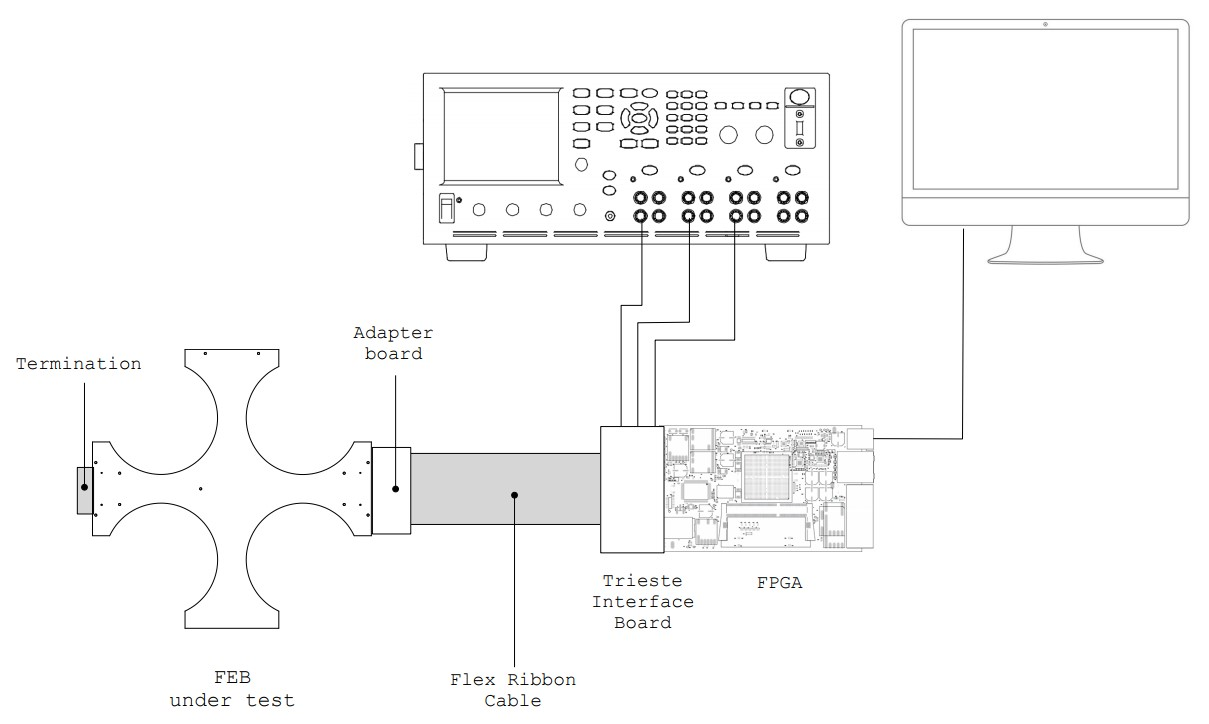
\includegraphics[width=0.95\textwidth]{Images/chap2/test_setup_FEB_1.jpg}
    \caption{Depiction of the setup adopted for the tests on the first set of FEBs.}
    \label{figFEBtest1}
\end{figure}

\begin{figure}[h!]
    \centering
    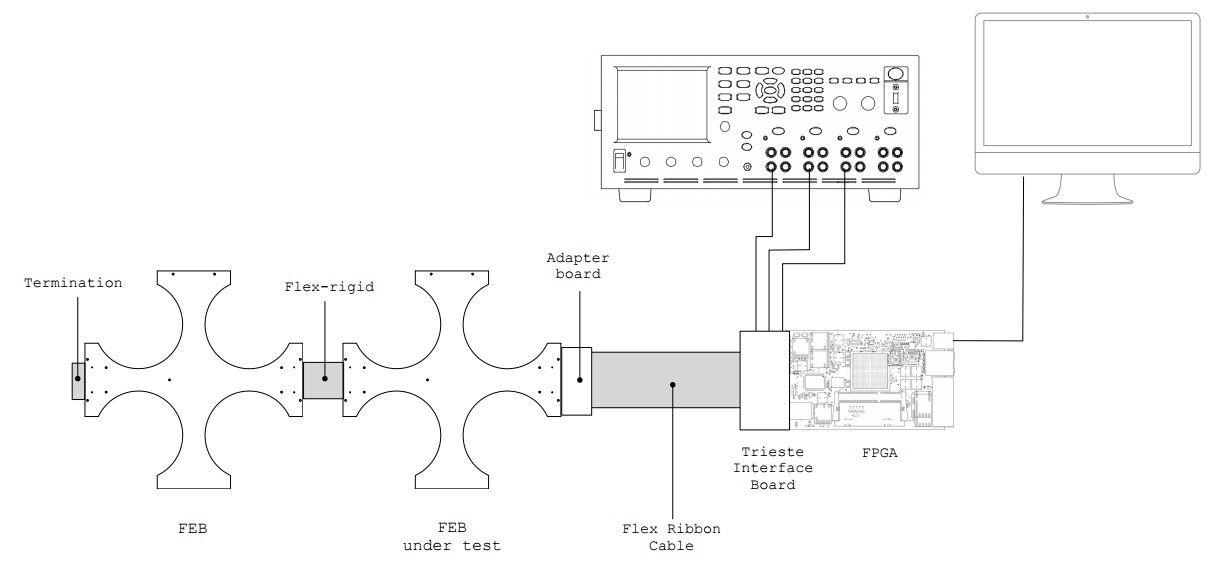
\includegraphics[width=0.95\textwidth]{Images/chap2/test_setup_FEB_2.jpg}
    \caption{Depiction of the improved setup adopted for the tests of the FEBs.}
    \label{figFEBtest2}
\end{figure}

\begin{itemize}
    \itemsep0em 
    \item Two front-end boards, each of which has a SLIDER32 ASIC onboard, as described in \hyperref[secGAPSfrontend]{Appendix \ref{secGAPSfrontend}}.
    \item A flex-rigid board, later described in \hyperref[flexrigids]{Section \ref{flexrigids}}, connecting the two FEBs.
    \item A Keysight N6705C DC Power analyser providing both analog and digital supply voltages to the FEB, with the same configuration as the one already discussed in \mbox{\hyperref[testboardsetup]{Section \ref{testboardsetup}}}.
    \item A flex ribbon cable connecting the interface board to the main test board.
    \item An adapter board connecting the FEB trough its female ERNI connector (model \texttt{354178}) to the flex ribbon cable.
    \item An ALTERA Cyclone V Field Programmable Gate Array (FPGA) programmed using Verilog, an Hardware Description Language (HDL) that allows to describe digital electronic systems. The FPGA sends Serial Peripheral Interface (SPI) commands to the FEB according to those expected by the ASIC digital back-end, listed in \hyperref[tabSPIcommand]{Table \ref{tabSPIcommand}}, that are propagated through all the connected FEBs by means of the flex-rigid boards.
    \item An interface board specifically designed to route the power supplies and the signals trough the flex ribbon cable to the front-end board under test.
    \item A PC running a Python-based testing program called \texttt{GAPS\_ModuleTester}, currently in its 4th version, connected to the FPGA via two Universal Serial Bus (USB) cables. This software has been specifically developed to perform a series of tests on the SLIDER32 ASIC and it is later described in \hyperref[sec21]{Section \ref{sec21}}.
\end{itemize}

% descrizione software python
\noindent
In order for the FPGA to be programmed, the software Intel Quartus Prime is used to upload the firmware onto the FPGA. After that, the \texttt{GAPS\_ModuleTester} Python program is run so as to perform a full automated test of the FEB in all its functionalities. This software allows to set global variables related to the SPI and the ADC clock frequencies, expressed in \SI{}{\mega\hertz}, the time limit for the self-trigger mode and the events delay generated by the FPGA, expressed in FPGA clock. The program offers three main interfaces, shown in \hyperref[figmodtest]{Figure \ref{figmodtest}}.

\begin{figure}[h!]
    \centering
    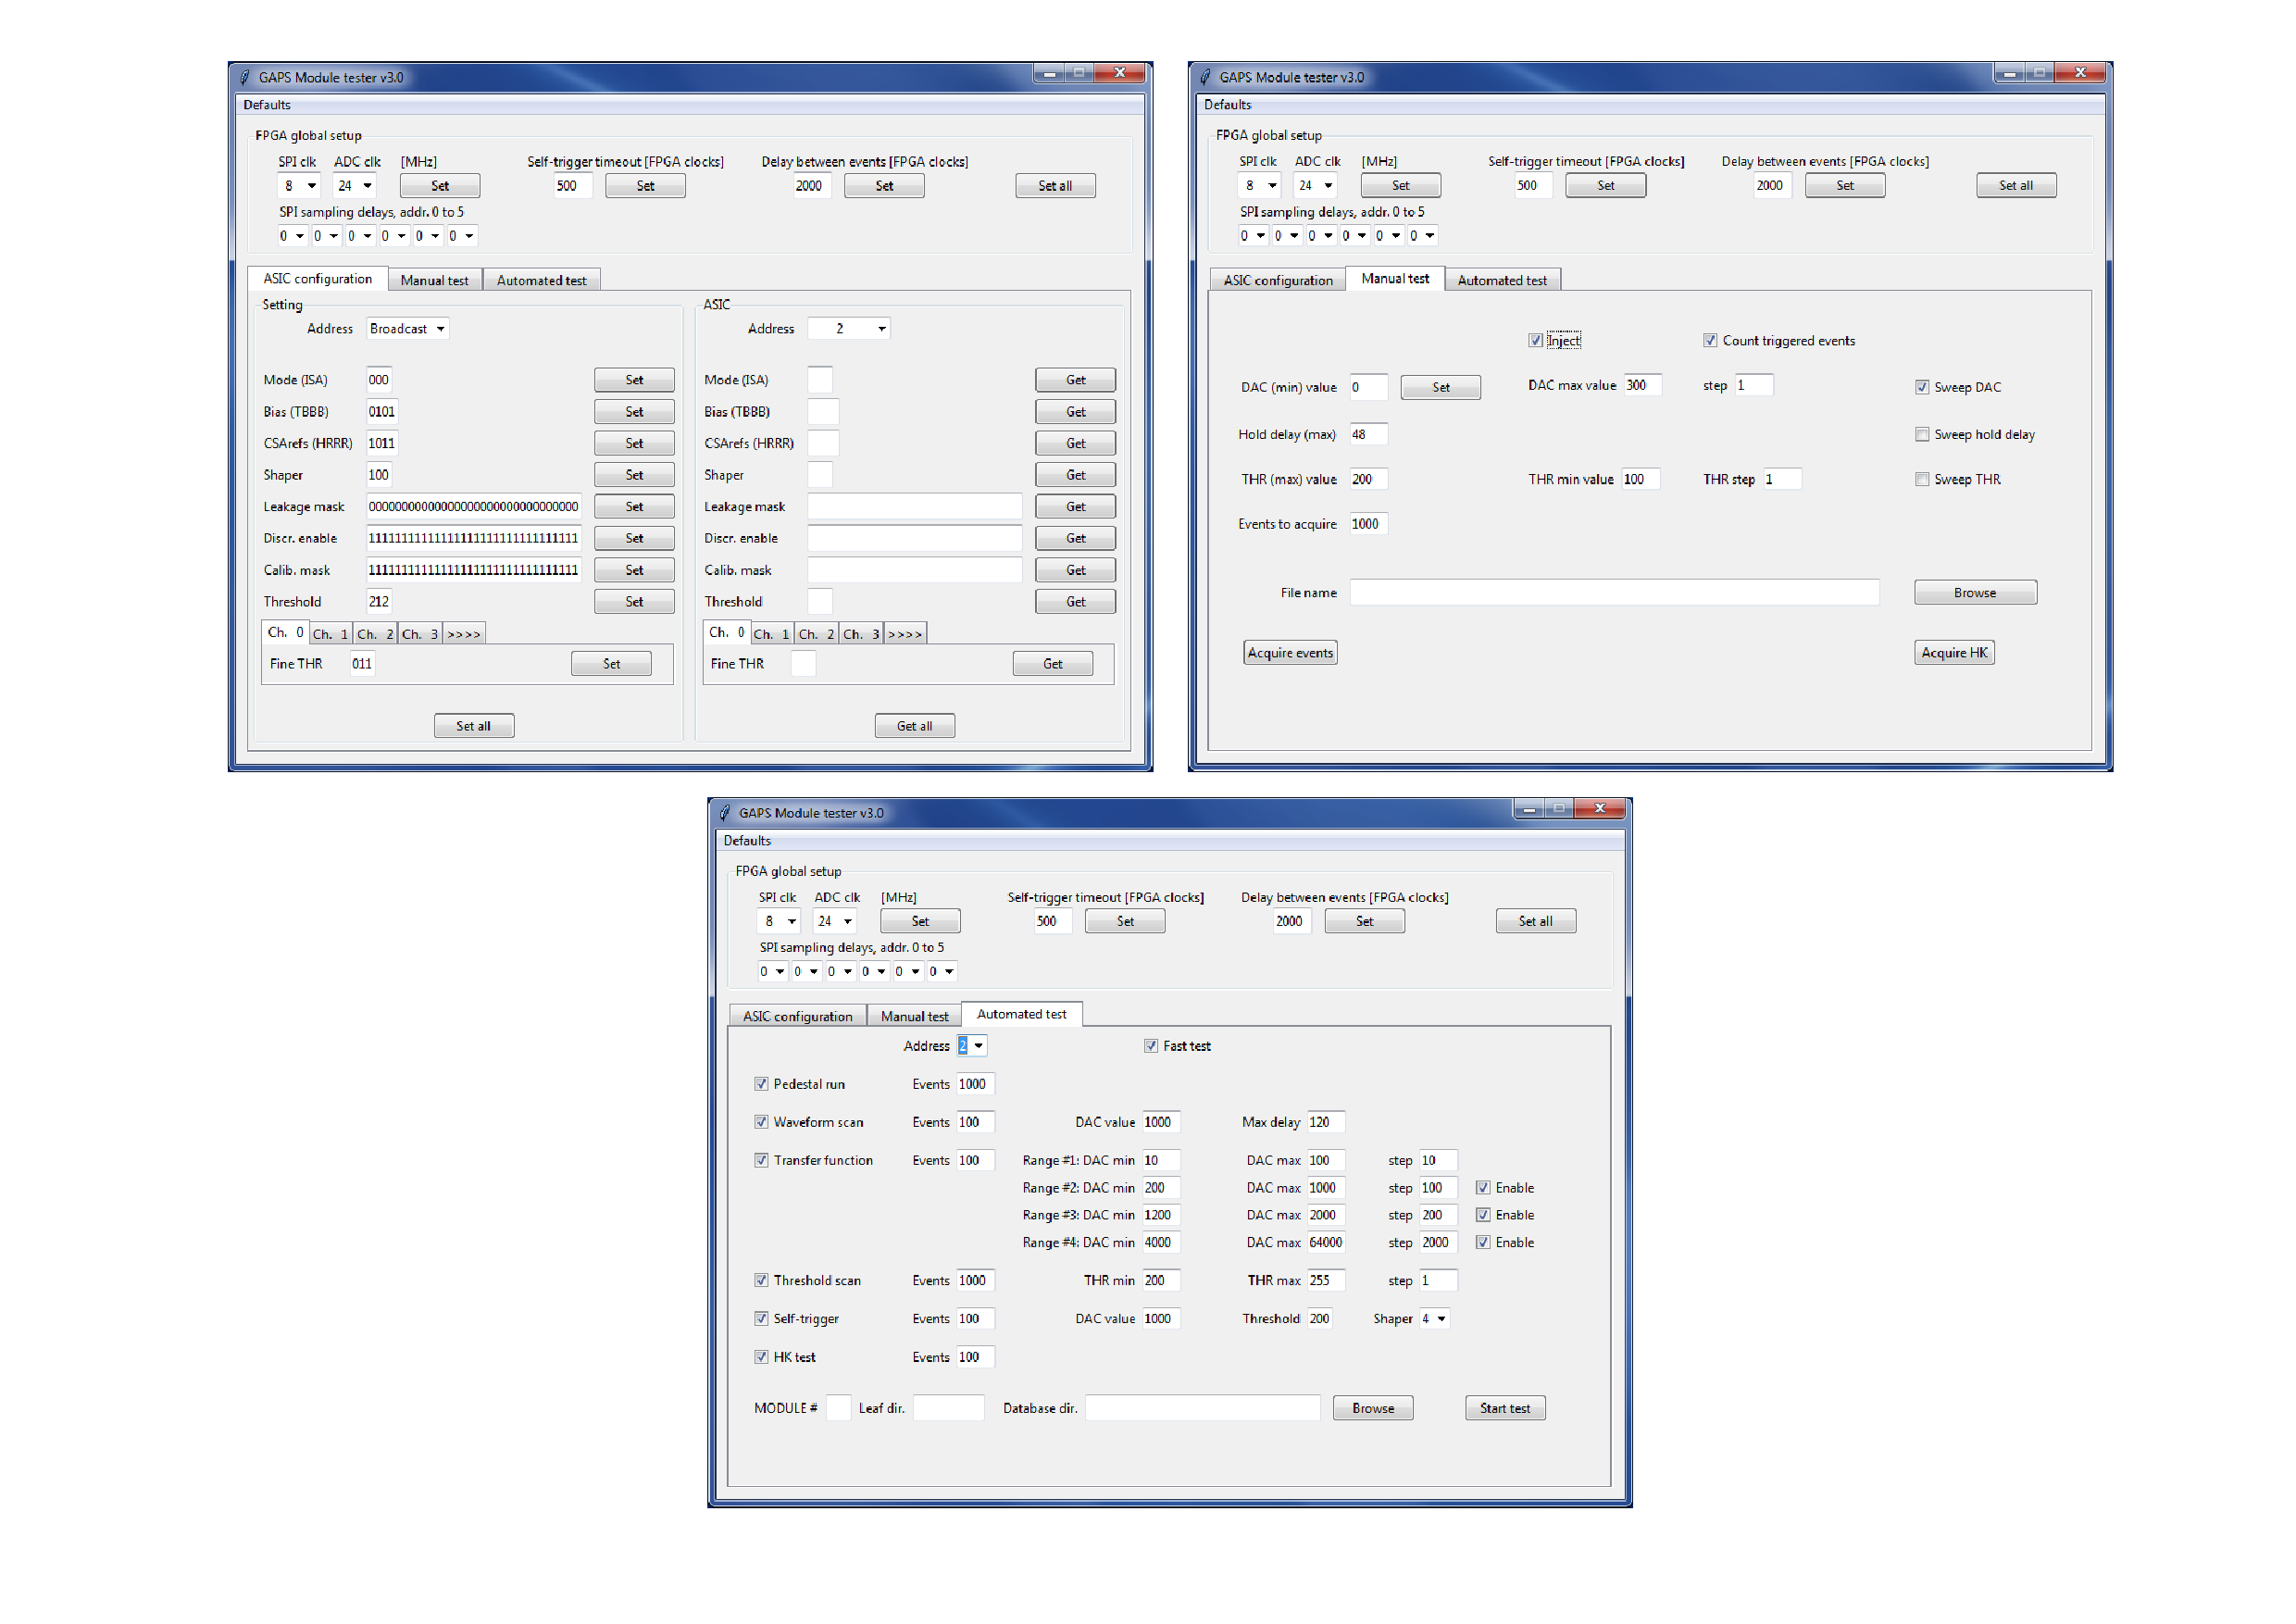
\includegraphics[width=0.97\textwidth]{Images/chap2/moduletester.pdf}
    \caption{\texttt{GAPS\_ModuleTester} main interfaces (clockwise from top-left): ASIC configuration, Manual Test, Automated Test.}
    \label{figmodtest}
\end{figure}

\par
The first interface, called \textit{ASIC configuration}, is dedicated to the configuration of the ASIC, namely its address, registers and configuration bits, specifically:

\begin{enumerate}
    \itemsep0em 
    \item OPERATING MODE (\texttt{ISA} bit);
    \item GLOBAL BIAS REGULATION (\texttt{TBBB} bits); %, where bit \texttt{T} is not used in SLIDER32);
    \item CSA REFERENCE REGULATION (\texttt{HRRR} bits, where bit \texttt{H} is set to \texttt{1} at ambient temperature and \texttt{0} at \SI{-40}{\celsius});
    \item SHAPER TIME CONSTANT (\texttt{TTT} bit);
    \item DISCRIMINATOR ENABLE MASK (32 bit mask for channel activation);
    \item LEAKAGE CURRENT MASK (for leakage current measurements);
    \item CALIBRATION MASK (for calibration purposes).
\end{enumerate}

\noindent
Through this interface it is also possible to set the global threshold (DISCRIMINATOR THRESHOLD, 8 bit) and the fine threshold for each channel (FINE THRESHOLD, 3 bit). A detailed description of the aforementioned configuration bits can be found in \hyperref[tabSPIcommand]{Table \ref{tabSPIcommand}} that presents the SPI commands accepted by the digital section of the ASIC. 

\par
The \textit{Manual test} interface allows to configure all parameters in order to perform a manual test, like the 16-bit DAC values range for injection (expressed in DAC units), the time interval between injections (expressed in FPGA clocks, where one FPGA clock is equivalent to $\approx \SI{20.83}{\nano\second}$, since the FPGA operates at a frequency of \SI{48}{\mega\hertz}) and the number of events to acquire. It is also necessary to set the output folder path which will contain the configuration parameters and the data generated by the test itself.

\begin{table}[h!]
    \centering
    \resizebox{1\columnwidth}{!}{
        \begin{tabular}{l l l l} 
            \Xhline{2\arrayrulewidth}
            Command name & Command code & Input data & Output data \T\B \\
            \hline
            READ EVENT DATA & \texttt{00000xxx} & $\minus$ & Event data packet \T\B \\
            READ SEU FLAGS/TEMPERATURE SENSOR & \texttt{00001xxx} & $\minus$ & SEU \& Temperature word \T\B \\
            READ OPERATING MODE & \texttt{00010xxx} & $\minus$ & \texttt{00000ISA} \T\B \\
            READ SHAPER TIME CONSTANT & \texttt{00011xxx} & $\minus$ & \texttt{00000TTT} \T\B \\
            READ CSA REFERENCE REGULATION & \texttt{00100xxx} & $\minus$ & \texttt{0000HRRR} \T\B \\
            READ GLOBAL BIAS REGULATION & \texttt{00101xxx} & $\minus$ & \texttt{0000TBBB} \T\B \\
            READ LEAKAGE CURRENT MASK & \texttt{00111xxx} & $\minus$ & 32 bit word \T\B \\
            READ DISCRIMINATOR ENABLE MASK & \texttt{01000xxx} & $\minus$ & 32 bit word \T\B \\
            READ CALIBRATION MASK & \texttt{01001xxx} & $\minus$ & 32 bit word \T\B \\
            READ DISCRIMINATOR THRESHOLD & \texttt{01010xxx} & $\minus$ & \texttt{DDDDDDDD} \T\B \\
            READ FINE THRESHOLD ADJ. CH. \texttt{NNNNN} & \texttt{011NNNNN} & $\minus$ & \texttt{00000FFF} \T\B \\
            WRITE OPERATING MODE & \texttt{10010ISA} & $\minus$ & $\minus$ \T\B \\
            WRITE SHAPER TIME CONSTANT & \texttt{10011TTT} & $\minus$ & $\minus$ \T\B \\
            WRITE CSA REFERENCE REGULATION & \texttt{v10100xxx} & \texttt{0000HRRR} & $\minus$ \T\B \\
            WRITE GLOBAL BIAS REGULATION & \texttt{10101xxx} & \texttt{0000TBBB} & $\minus$ \T\B \\
            SET CALIBRATION DAC VOLTAGE & \texttt{10110xxx} & 16 bit word & $\minus$ \T\B \\
            WRITE LEAKAGE CURRENT MASK & \texttt{10111xxx} & 32 bit word & $\minus$ \T\B \\
            WRITE DISCRIMINATOR ENABLE MASK & \texttt{v11000xx}x & 32 bit word & $\minus$ \T\B \\
            WRITE CALIBRATION MASK & \texttt{11001xxx} & 32 bit word & $\minus$ \T\B \\
            WRITE DISCRIMINATOR THRESHOLD & \texttt{11010xxx} & \texttt{DDDDDDDD} & $\minus$ \T\B \\
            WRITE FINE THRESHOLD ADJ. CH. \texttt{NNNNN} & \texttt{111NNNNN} & \texttt{00000FFF} & $\minus$ \T\B \\
            \Xhline{2\arrayrulewidth}
        \end{tabular}
    }
    \caption{SPI commands and configuration bits.}
    \label{tabSPIcommand}
\end{table}

\par
The last section concerns the \textit{Automated test} that has been used in order to perform the validation of the front-end boards. The automated test carried out on each FEB generates a folder containing the raw data acquired from the board, in the form of \texttt{.dat} files, and it has the following structure.\\

\vspace{-0.3cm}
\dirtree{%
.1 MODULE\_000\_fast/.
.2 1/.
.2 data/.
.3 ConfigurationTest.dat.
.3 HK\_Leakage\_chX.dat.
.3 Pedestal\_tauY.dat.
.3 SelfTrigger\_chX.dat.
.3 ThresholdScan\_fthrZ\_tauY.dat.
.3 TransferFunction\_fast\_tauY.dat.
.3 WaveformScan\_fast\_tauY.dat.
} 

\noindent
where \texttt{X} represents the channel identifier number that spans from 0 to 31, while \texttt{Y} represents the peaking time, that goes from 0 to 7. Specifically, the content of each of the files is defined as follows.

\begin{enumerate}
    \itemsep0em 
    \item \texttt{ConfigurationTest.dat}: Basic communication and configuration tests.
    \item \texttt{HK\_Leakage\_chX.dat}: Leakage current measurement (to be done with detectors).
    \item \texttt{Pedestal\_tauY.dat}: Pedestal test, in which the baseline variations due to electronic noise are measured. This test evaluates the electronic noise within the channel, measuring its output without injecting any charge. The output signal is therefore purely attributable to noise.
    \item \texttt{SelfTrigger\_chX.dat}: Self-trigger measurement, which reports the output of the ASIC channel (in ADU) obtained with a fixed DAC injection code and using the automatic peak detection feature of the Zero Crossing circuit, described in \hyperref[zeroCrossing]{Appendix \ref{zeroCrossing}}.
    \item \texttt{ThresholdScan\_fthrZ\_tauY.dat}: Threshold measurement, which reports the number of comparator hits, obtained by varying the global threshold word over its range and injecting 1000 times with a fixed DAC code at each step.
    \item \texttt{TransferFunction\_fast\_tauY.dat}: Transfer function measurement, which lists the channel output ADC code obtained by sweeping the calibration DAC code over its range.
    \item \texttt{WaveformScan\_fast\_tauY.dat}: Waveform scan, which reports the output ADC code sampled at delayed times making possibile to reconstruct the shaper transient response.
\end{enumerate}

\noindent
After the data acquisition process, a MATLAB script is run in order to analyse and plot all the tests results, and the output folder has the following structure.\\

\vspace{-0.3cm}
\dirtree{%
.1 MODULE\_000/.
.2 1/.
.3 analysis\_matlab/.
.4 ENC/.
.4 Pedestal/.
.4 SelfTrigger/.
.4 ThresholdScan/.
.4 TransferFunction/.
.4 WaveformScan/.
} 

\noindent
Each sub-directory contains the following:

\begin{enumerate}
    \itemsep0em 
    \item \texttt{ENC}: Equivalent Noise Charge (ENC) elaborated data and plots obtained from pedestal and transfer function (high gain) processing.
    \item \texttt{Pedestal}: Pedestal elaborated data and plots representing the dispersion of the baseline due to electronic noise.
    \item \texttt{SelfTrigger}: Self trigger plots (histograms) representing dispersion of the value read at the output of the ADC triggered by the Zero Crossing circuit.
    \item \texttt{ThresholdScan}: Threshold scan elaborated data and plots reporting the statistics on the threshold obtained through fitting the data with an error function and a threshold dispersion minimisation analysis.
    \item \texttt{TransferFunction}: Transfer function elaborated data and plots, representing channel input/output characteristic.
    \item \texttt{WaveformScan}: Waveform scan elaborated data and plots representing the shaper transient response.
\end{enumerate}

%-------------------------------------------------------------------------------

\subsection{Visual inspection} \label{FEBdefects}

A manual visual inspection has been performed on each FEB by looking over the board either with the naked eye or through magnification. The board has been compared to the design documents to ensure that all specifications were met. The purpose of this activity was to look for common defaults (missing or bad-soldered components) and defects (pits, dents, scratches, pinholes and other defects on printing traces and pads). If no or negligible defects were found, \texttt{[YES]} has been reported in the \textit{Visual Inspection} field of the test report module, similar to the one shown in \hyperref[figF065I]{Figure \ref{figF065I}}. If a missing or bad-soldered component was found, the board was reworked and the operation has been reported in the \textit{Notes} section of the report. A brief description of the most common visual defects that have been categorised is available in \hyperref[figScratches]{Figure \ref{figScratches}}.

\begin{figure}[ht]
    \centering
    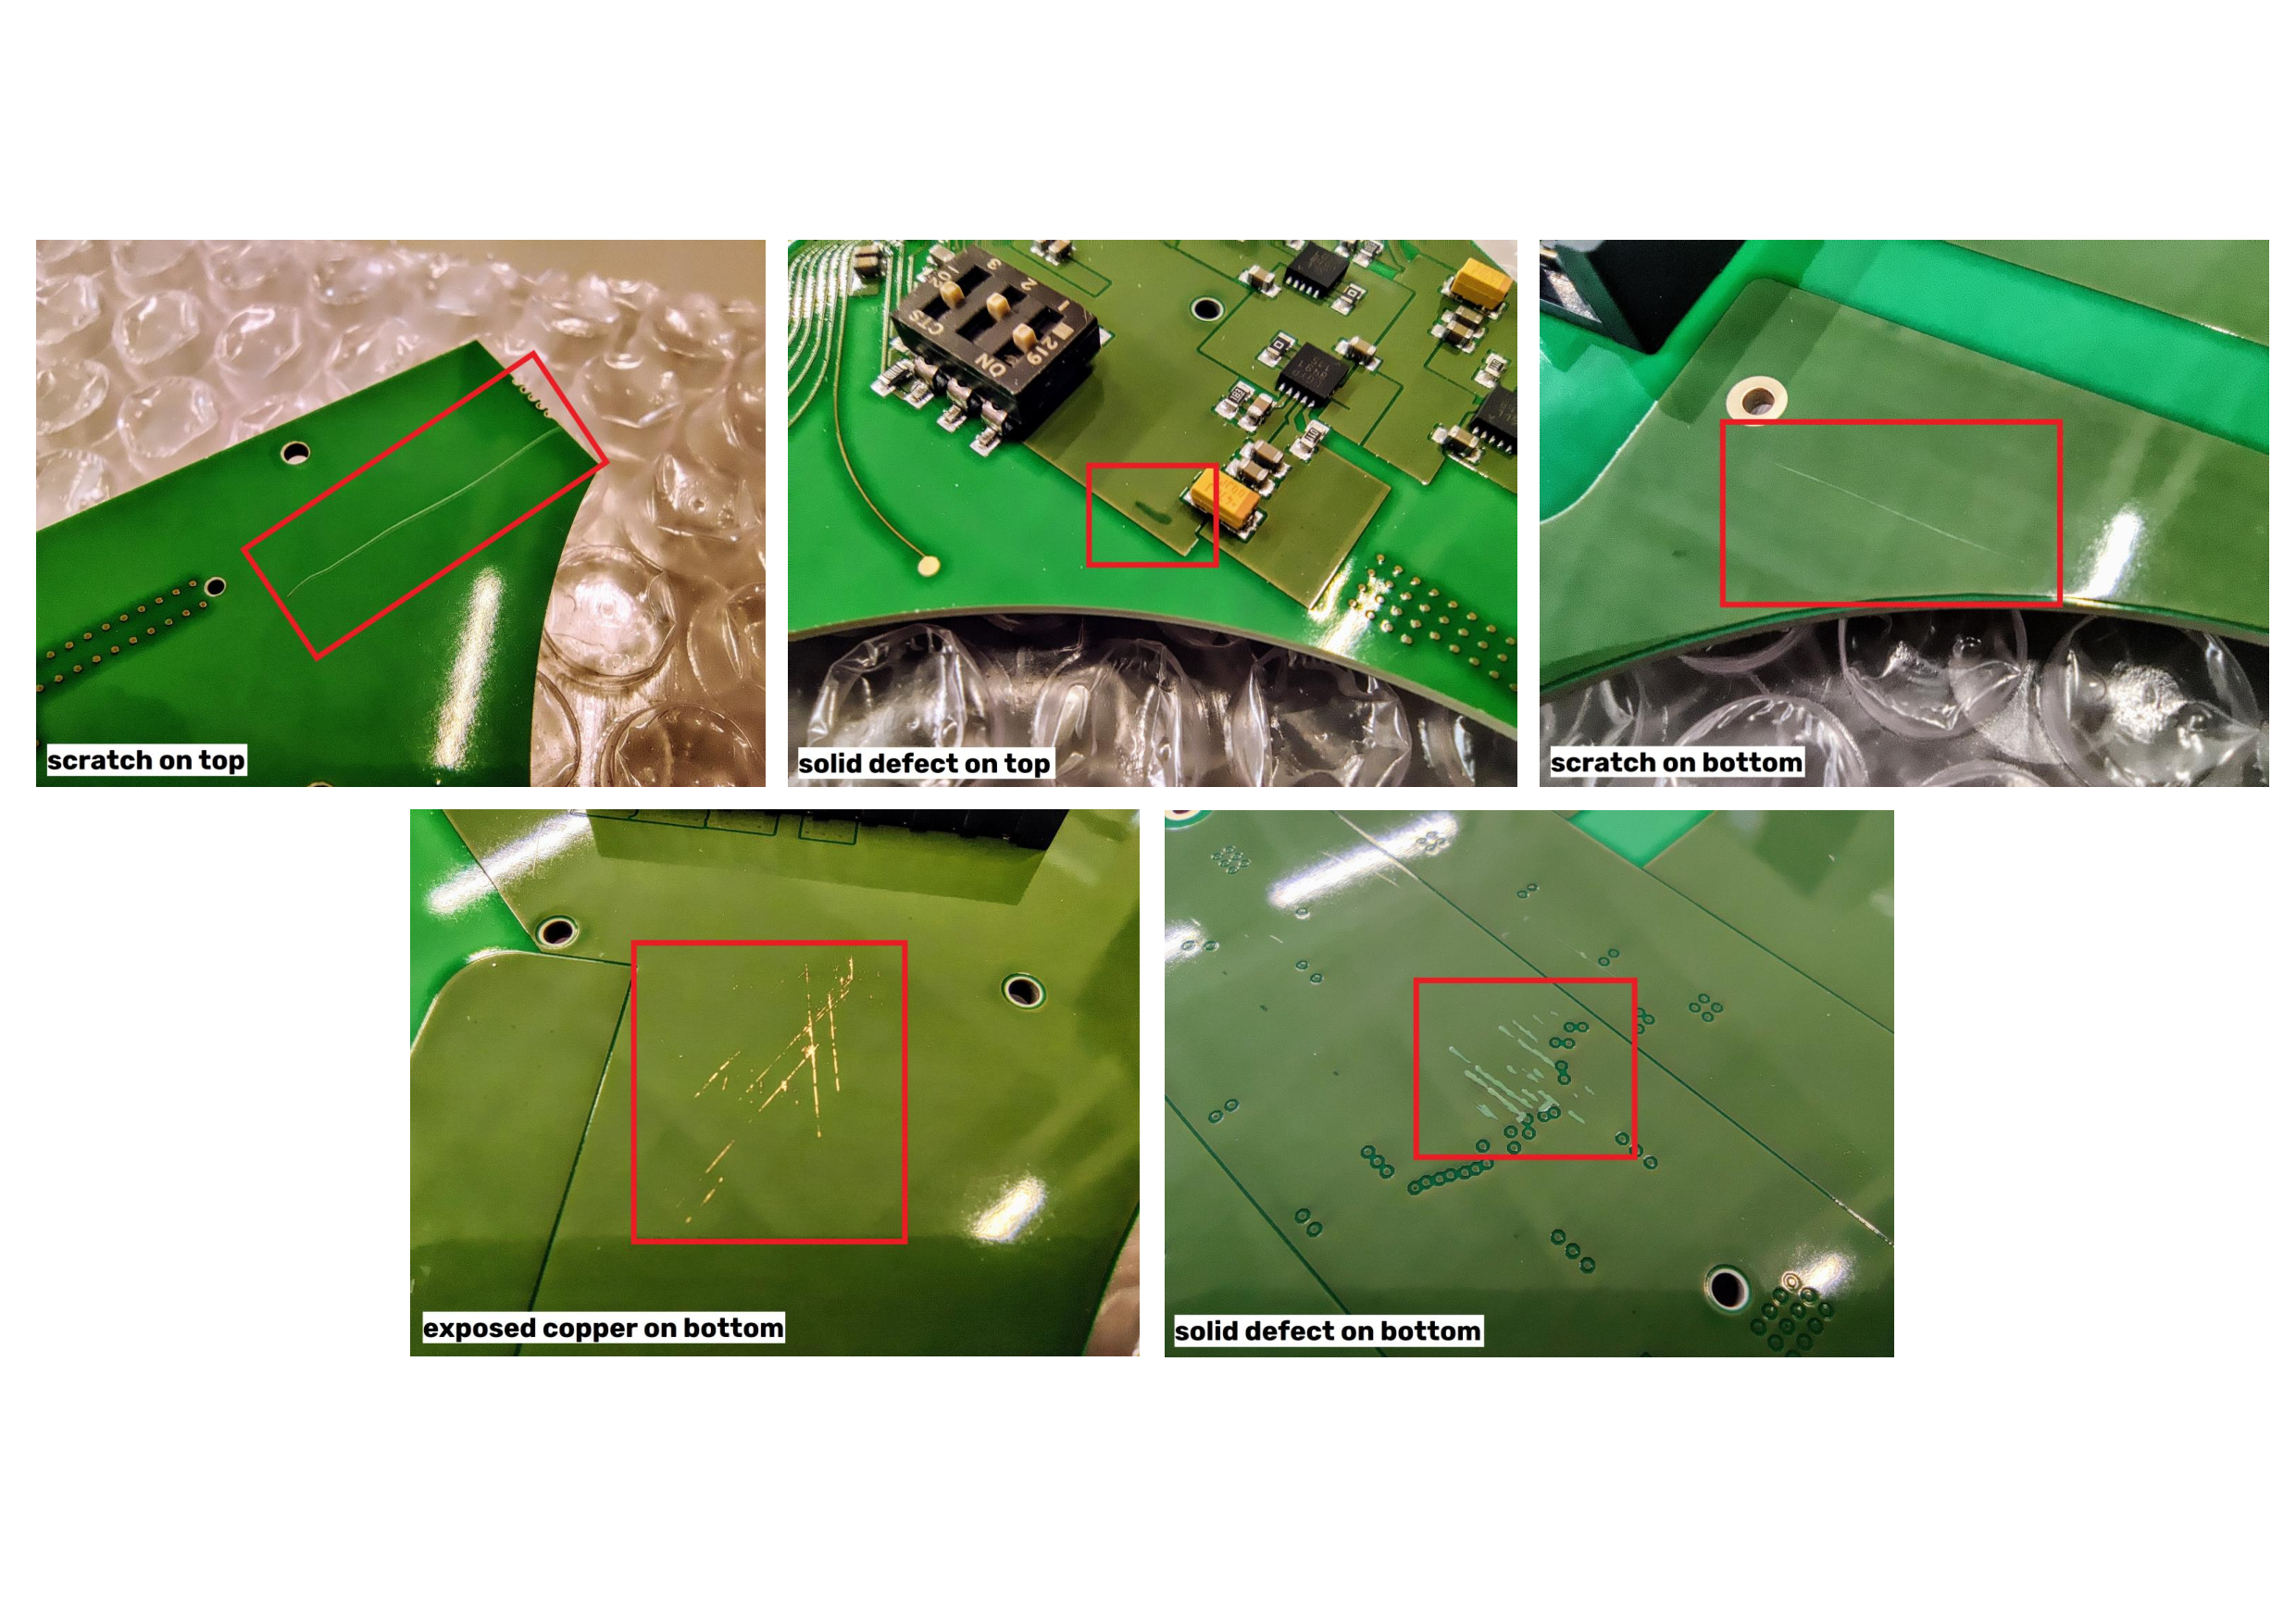
\includegraphics[width=1\textwidth]{Images/chap2/immagini_difetti.pdf}
    \caption{Examples of defects found during visual inspection of the FEBs (clockwise from top-left): scratch on top, solid defect on top, scratch on bottom, exposed copper on bottom, solid defect on bottom.}
    \label{figScratches}
\end{figure}

\par
It is important to emphasise the fact that the visual analysis to search for defects on the board or the components installed on it was of paramount importance in identifying problems that could have altered the proper functioning of the FEB. For example, if there was exposed copper in contact with other metals on the board, short circuits could possibly occur. Furthermore, in the event that a defect in one of the metal layers of the board was very large, this could result in a change in the resistance value of the entire metal layer (e.g. a power supply or a ground), thereby affecting the power consumption and thus altering the nominal operation of the board. In the event that one of the aforementioned defects led to the partial or total non-functioning of the board, the latter was categorised as "reworked" and separated from the others. %A total of 8 FEBs of Italian production and 2 of the US production were classified in this way and are intended to be used for testing purposes only.

%-------------------------------------------------------------------------------

\subsection{Bias} \label{bias}

In this test, the DC voltages are measured with a Fluke 79 III digital multimeter and the DC currents are monitored with the built-in amperometer of the Keysight N6705C
DC Power analyser used as power supply. The only exception is for the Ibias current that is derived from the voltage drop on a \SI{100}{\ohm} Surface Mounted Device (SMD) test resistor (\SI{0.1}{\percent} precision) on the FEB. During the test the ASIC is biased with the following configuration: \texttt{TBBB=0101} and \texttt{HRRR=1011}. The DC voltage and DC current measurements are reported respectively in \hyperref[tabvoltages]{Table \ref{tabvoltages}} and \hyperref[tabcurrents]{Table \ref{tabcurrents}}.

\par
For these measurements, the pass/fail criterion is not obvious, so the typical measurement value has been determined iteratively by analysing the results of the measurements carried out on a larger number of boards, whose test results can be found in \hyperref[FEBresults]{Section \ref{FEBresults}}. If a value in the range of $\pm \SI{10}{\percent}$ with respect to the mean was obtained, \texttt{[YES]}
has been reported in the corresponding section of the report.

\begin{table}[ht]
    \centering
    \begin{tabular}{l l l} 
         \Xhline{2\arrayrulewidth}
         Voltage & Nominal & Description \T\B \\
         \hline
         AVDD & \SI{1.80}{\volt} & \makecell[l]{Voltage at the output of the LDO that regulates the  \T \\ (ASIC) analog power supply \B} \\ 
         DVDD & \SI{1.80}{\volt} & \makecell[l]{Voltage at the output of the LDO that regulates \T the \\ (ASIC) digital power supply \B} \\ 
         3V3 & \SI{3.00}{\volt} & \makecell[l]{Voltage at the output of the LDO that regulates \T the \\ (ASIC) calibration power supply \B} \\ 
         VCMSH & \SI{1.20}{\volt} & Reference voltage for the S\&H \T\B \\ 
         VCM & \SI{0.88}{\volt} & Reference voltage for the shaper \T\B \\ 
         RVCM & \SI{0.90}{\volt} & Reference voltage for the ADC \T\B \\ 
         \Xhline{2\arrayrulewidth}
    \end{tabular}
    \caption{List of voltages measured during the bias test of the FEB.}
    \label{tabvoltages}
\end{table}

\begin{table}[ht]
    \centering
    \begin{tabular}{l l l} 
         \Xhline{2\arrayrulewidth}
         Current & Nominal & Description \T\B \\
         \hline
         IAVDD & \SI{136}{\milli\ampere} & \makecell[l]{Current absorbed by the LDO that regulates the (ASIC) \T \\ analog power supply \B} \\
         IDVDD & \SI{4}{\milli\ampere} & \makecell[l]{Current absorbed by the LDO that regulates the (ASIC) \T \\ digital power supply \B} \\ 
         I3V3 & \SI{3}{\milli\ampere} & \makecell[l]{Current absorbed by the LDO that regulates the (ASIC) \T \\ calibration power supply \B} \\ 
         Ibias & \SI{5}{\milli\ampere} & Bias current for the CSA \T\B \\ 
         \Xhline{2\arrayrulewidth}
    \end{tabular}
    \caption{List of currents measured during the bias test of the FEB.}
    \label{tabcurrents}
\end{table}

%-------------------------------------------------------------------------------

\subsection{Digital}

In this Section of the test report document, results coming from the \textit{Automated test} of the \texttt{GAPS\_ModuleTester} software  are reported considering the following aspects:

\begin{itemize}
    \itemsep0em 
    \item \textbf{Configuration test}: It checks the capability to write and read registers of the digital back-end section of the ASIC of the board under tests. For the FEBs where the improved setup shown in \hyperref[figFEBtest2]{Figure \ref{figFEBtest2}} has been used, this test also accounts for the capability to communicate with the second FEB in the chain.
    \item \textbf{Wrong address test}: It checks the capability of the ASIC to ignore commands when an address, different to the one hardware coded on the board, is selected.
    \item \textbf{Temperature sensor}: It verifies the response of the ADC when the sensor temperature of the FEB is readout.
    
\end{itemize}

%-------------------------------------------------------------------------------

\subsection{Analog}
\label{FEBanalogtest}
The results reported in this Section of the test report document are relevant to the performance of the analog readout channels of the ASIC. Data is obtained from the \textit{Automated test} of the \texttt{GAPS\_ModuleTester} software. The four main reference tests chosen to be included in the report are listed below.

\paragraph{Channel Input-output characteristic} The purpose of this test is to verify that all the channels respond to the input injected signal and provide the expected input-output characteristic with dynamic signal compression. If zero non-responding channels were found, \texttt{[YES]} has been reported in the \textit{Input-output characteristic} field of the test report document.

\paragraph{Noise} The noise performance of 6 channels (No. 0, 7, 15, 16, 23 and 31) is expressed in terms of ENC FWHM in \SI{}{\kilo\electronvolt} and results obtained for peaking time \#6 are reported in this Section. Since the measurement conditions of the FEB are not optimised from a noise point of view, it is not expected that the channels provide the minimum ENC. Therefore, a value lower than \SI{200}{\kilo\electronvolt} is considered good enough to have a \texttt{[YES]} assigned. In the case of 135 US-made FEBs, the ENC measurement was carried out by placing the board inside a metal box in order to shield it from any electromagnetic interference present in the measurement environment. In this way, it was possible to measure ENC values that could provide a more faithful representation of the board actual noise performance. The ENC measurements for 6 of the 32 channels of the ASIC are shown in \hyperref[figFEBNoise]{Figure \ref{figFEBNoise}}.

\paragraph{Threshold dispersion} The threshold dispersion of the 32 channels of the ASIC is reported here, before and after the fine trimming procedure that is adopted to minimise the dispersion of the threshold distribution. This test is conducted in order to determine the width (i.e. the standard deviation) of the distribution of threshold values associated with the 32 channels of the readout electronics. In fact, each channel has a threshold value associated with the minimum energy level at which the comparator is triggered: due to variations in the manufacturing process of the transistors constituting the circuit blocks of the channel (a phenomenon known as \textit{transistor mismatch}), these may in fact have associated threshold values lower or higher than the one specified. The purpose of this test is therefore to check how far the threshold value disperses around the set value. The purpose of this test is also to verify the effectiveness of the 3-bit ADC in each channel used to fine-tune the threshold and thus reduce its dispersion.

\paragraph{Pedestal dispersion} The distribution of the pedestal of the 32 readout channels is reported in this Section.\\

\par
Each FEB has been numbered using an alphanumerical identifier, allowing the board to be uniquely recognised during the assembly of the tracker. The identifier number is composed of three parts, as shown below.

\begin{gather*}
    %\useshortskip
    \Large
    \smallunderbrace{\mathrm{F}}_{\text{\clap{1}}} 
    \smallunderbrace{\mathrm{065}}_{\text{\clap{2}}}
    \smallunderbrace{\mathrm{I}}_{\text{\clap{3}}}
\end{gather*}

\noindent
Specifically, each part of the alphanumerical sequence serves the purpose of:

\begin{enumerate}
    \itemsep0em 
    \item \textbf{F}: It classifies the component ("F" as for "Flight", meaning the FEB has installed a SLIDER32 ASIC in the version intended for use in the in-flight experiment).
    \item \textbf{065}: It uniquely represents the specific board via an increasing numerical value, which matches the numerical identifier of the SLIDER32 ASIC installed on the front-end board.
    \item \textbf{I}: It identifies the country of the manufacturer of the board ("I" for the Italian-made FEBs and "U" for the US-made ones).
\end{enumerate}

\par
For each FEB tested, a test report has been generated in order to sum up all the information regarding the whole testing activity carried out on the front-end board. An example of the aforementioned test report is shown in \hyperref[figF065I]{Figure \ref{figF065I}}. 

\normalsize

%-------------------------------------------------------------------------------

\subsection{GAPS-FEB-Report-Generator}
This Section provides a brief description of the Python software that has been developed in order to automatically generate the test reports for the FEBs, as the one shown in \hyperref[figF065I]{Figure \ref{figF065I}}. The code can be found on GitHub at the following \href{https://github.com/lucaghislo/GAPS-FEB-report-generator}{\underline{link}}.

\subsubsection{Software functionalities} \label{GAPSrepfun}
The software works by taking as input two Comma Separated Values (CSV) files reporting the voltage and current measurements taken on the FEBs and the corresponding defects that have been found during the visual inspection, including optional notes, and producing a report summarising all the data both as a Microsoft Word document and a Portable Document Format (PDF) file, the contents of which are shown in \hyperref[figF065I]{Figure \ref{figF065I}}.\\

\noindent
The Python code is basically organised in two parts:

\begin{enumerate}
    \itemsep0em
    \item \texttt{FEB\_report\_fun.py}: It contains all the functions that are used in order to fill in the Word document and to export the corresponding PDF file. This file also contains the functions used to export log files and CSV tables containing a summary of the values obtained during the testing of each individual FEB.
    \item \texttt{FEB\_report\_out.py}: It contains the function calls to the function blocks defined in the previous file and uses them to build the output document.
\end{enumerate}

%-------------------------------------------------------------------------------

\subsubsection{Software structure}
The software is organised into different sub-folders, each one containing specific input or output files, as described in the following directory tree:\\

\vspace{-0.3cm}
\dirtree{%
.1 GAPS-FEB-report-generator/.
.2 configuration/.
.3 config.conf.
.2 CSV\_tables/.
.3 FEB\_testing - Defects.csv.
.3 FEB\_testing - Multimeter.csv.
.2 modules/.
.3 MODULE\_000/.
.3 ....
.2 output/.
.3 FEB\_report\_log.pdf.
.3 FEB\_report\_log.txt.
.3 script\_values.csv.
.3 temperature\_ADC.csv.
.3 temperature\_C.csv.
.2 report\_PDF/.
.3 F000I.pdf.
.3 ....
.2 report\_template/.
.3 test\_report\_FEB.docx.
.2 report\_word/.
.3 F000I.docx.
.3 ....
.2 script\_files/.
.3 FEB\_report\_fun.py.
.3 FEB\_report\_out.py.
}

\vspace{0.5cm}
\noindent
Moreover, each individual item serves the following function.

\begin{enumerate}
    \itemsep0em
    \item \texttt{config.conf}: Configuration file where the user can specify the nation identifier letter (\texttt{nation\_letter} field) of the producer of the board (\texttt{I} for Italy and \texttt{U} for US production), the document version (\texttt{doc\_version} field), the date, the author name and surname and the nationality of the manufacturer (\texttt{Italian} or \texttt{US}). 
    \item \texttt{FEB\_testing - Defects.csv}: CSV file containing a list of the defects found during the visual inspection of the FEBs, as discussed in \hyperref[FEBdefects]{Section \ref{FEBdefects}}.
    \item \texttt{FEB\_testing - Multimeter.csv}: CSV file containing the voltage and current measurements taken on the FEBs, as described in \hyperref[bias]{Section \ref{bias}}.
    \item \texttt{modules} folder: Containing the folders generated by the purposely developed MATLAB script, described in \hyperref[sec21]{Section \ref{sec21}}.
    \item \texttt{FEB\_report\_log.pdf} and \texttt{FEB\_report\_log.txt}: Log file containing a summary of all the reports fields presented in a single, multi-page document format.
    \item \texttt{script\_values.csv}: CSV file containing a summary of the values obtained during the evaluation of the performance of the analog readout channels of the ASIC generated by the \texttt{GAPS\_ModuleTester} testing software, as mentioned in \hyperref[FEBanalogtest]{Section \ref{FEBanalogtest}}.
    \item \texttt{temperature\_ADC.csv} and \texttt{temperature\_C.csv}: CSV files containing the readings of the temperatures in \SI{}{ADU} and \SI{}{\celsius} respectively.
    \item \texttt{report\_PDF/} folder: Folder containing the PDF version of the reports generated by the software.
    \item \texttt{test\_report\_FEB.docx}: Word template used to produce the final test reports in Word and PDF format.
    \item \texttt{report\_word/} folder: Folder containing the Word version of the reports generated by the software.
    \item \texttt{script\_files} folder: Folder containing the two main Python files used to implement the program, as described in \hyperref[GAPSrepfun]{section \ref{GAPSrepfun}}.
\end{enumerate}

\subsubsection{Software usage}
The program can be launched with Python 3 installed on the PC by double-clicking on the \texttt{FEB\_report\_out.py} Python file and by interacting with the command-line interface shown in \hyperref[figReportTerminal]{Figure \ref{figReportTerminal}}.

\begin{figure}[h!]
    \centering
    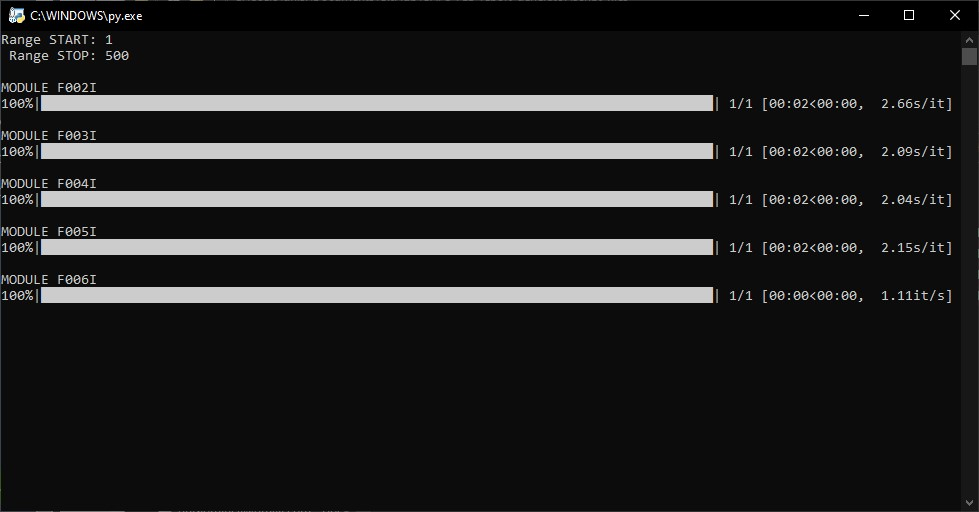
\includegraphics[width=0.8\textwidth]{Images/chap2/rep_gen_terminal.jpg}
    \caption{Command line interface of the \texttt{GAPS-FEB-report-generator} software.}
    \label{figReportTerminal}
\end{figure}

\par
At first, the software asks to input the minimum and maximum values of the FEB identifier numbers for which the user wants to generate a report. It has to be noted that for the program to be correctly executed, \texttt{FEB\_testing - Defects.csv} and \texttt{FEB\_testing - Mutltimeter.csv} have to be present in their corresponding folders. The report generation can be tracked through the loading bars showing the total time taken to compile each report. Once the generation of the reports is complete, the files can be found in \texttt{report\_word/} and \texttt{report\_PDF/} folders respectively.


%-------------------------------------------------------------------------------

\subsection{Analysis of test results} \label{FEBresults}

This Section describes the results of the measurements carried out during the validation phase of the front-end boards. Each graph shows the data distribution for the Italian-made front-end boards (in blue) and US-made ones (in red) separately for comparison purposes. 

\paragraph{AVDD and IAVDD} The graphs in \hyperref[figAVDDIVDD]{Figure \ref{figAVDDIVDD}} show the distributions of the analog supply voltage, AVDD, and the corresponding current IAVDD. The nominal value of AVDD, shown in \hyperref[tabvoltages]{Table \ref{tabvoltages}}, is \SI{1.80}{\volt}, while that of IAVDD, shown in \hyperref[tabcurrents]{Table \ref{tabcurrents}}, corresponds to \SI{136}{\milli\ampere}. It can be seen that both productions present an average voltage value comparable to the nominal one and have the same standard deviation. On the other hand, the average current value is below the nominal one for both productions, with the American one being on average \SI{1.49}{\percent} lower than expected and the Italian one reaching almost exactly the desired current value (\SI{135.93}{\milli\ampere} compared to the \SI{136.00}{\milli\ampere} nominal value).

\begin{figure}[ht]
    \centering
    \begin{tabular}{cc}
        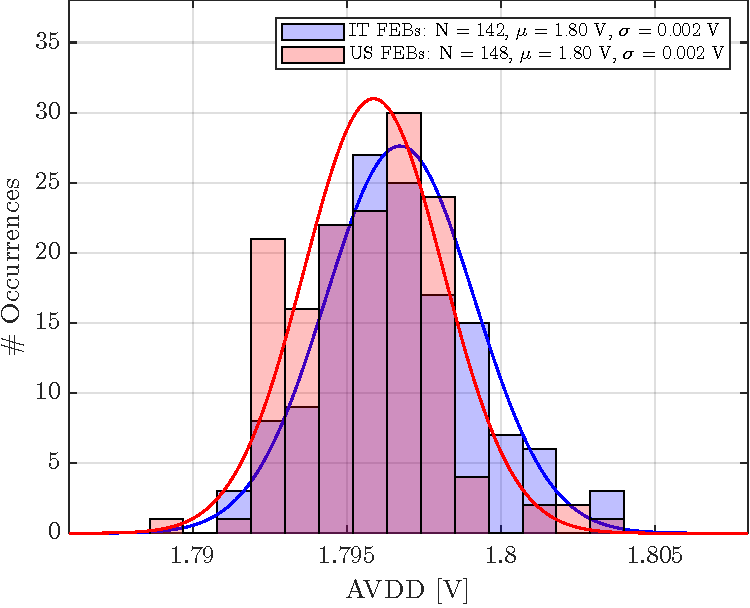
\includegraphics[width=0.475\textwidth]{Images/chap2/results/AVDD.pdf} & 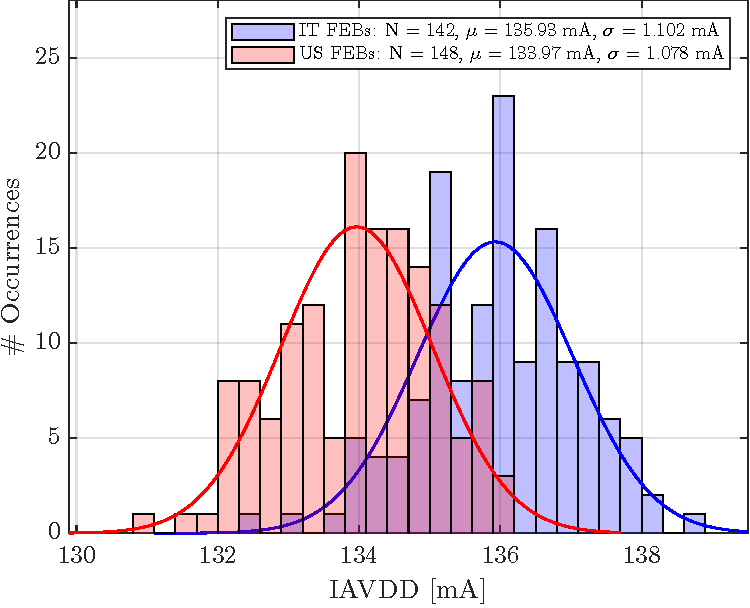
\includegraphics[width=0.475\textwidth]{Images/chap2/results/IAVDD.pdf}\\
    \end{tabular}
    \caption{AVDD values distribution, on the left, and IAVDD values distribution, on the right. Each histogram reports the mean value and standard deviation for both Italian and US productions.}
    \label{figAVDDIVDD}
\end{figure}

\paragraph{Ibias} \hyperref[figFEBIbias]{Figure \ref{figFEBIbias}} shows the distribution of the biasing current, Ibias, whose nominal value is \SI{5}{\milli\ampere}. For both productions, the average value of this parameter is almost comparable with the expected value, with a similar standard deviation between the two.

\begin{figure}[ht]
    \centering
    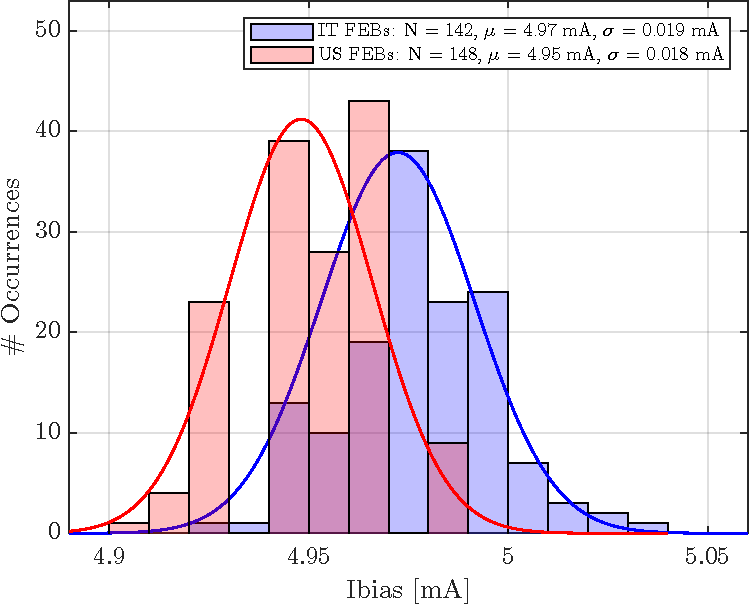
\includegraphics[width=0.475\textwidth]{Images/chap2/results/Ibias.pdf}
    \caption{Ibias values distribution. The histogram reports the mean value and standard deviation for both Italian and US productions.}
    \label{figFEBIbias}
\end{figure}

\paragraph{DVDD and IDVDD} In the case of the digital supply voltage DVDD and the respective current IDVDD, the distributions of the measured values are shown in \hyperref[figDVDDIDVDD]{Figure \ref{figDVDDIDVDD}}. As in the case of the analogue supply voltage, the average values of both outputs are comparable with the nominal value of \SI{1.80}{\volt}. As far as the current is concerned, in the case of the American production, a value of exactly \SI{5.00}{\milli\ampere} was found on all FEBs tested, resulting in a zero standard deviation.

\begin{figure}[h!]
    \centering
    \begin{tabular}{cc}
        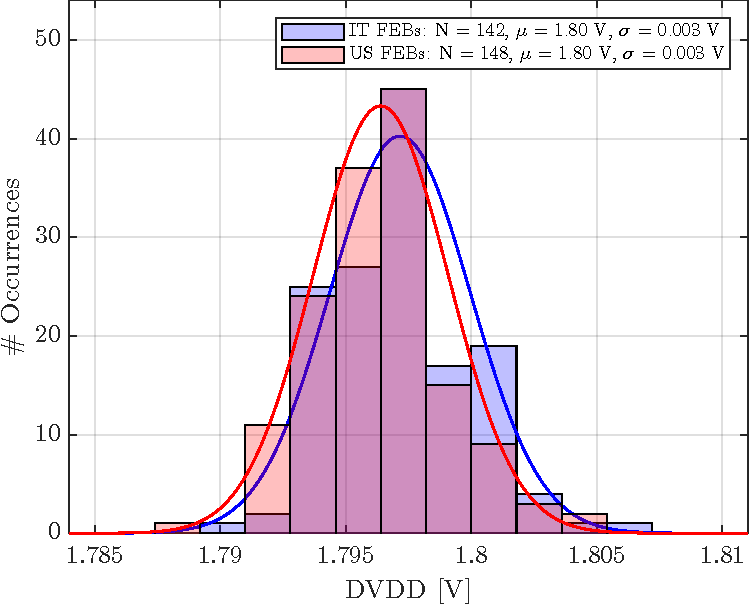
\includegraphics[width=0.467\textwidth]{Images/chap2/results/DVDD.pdf} & 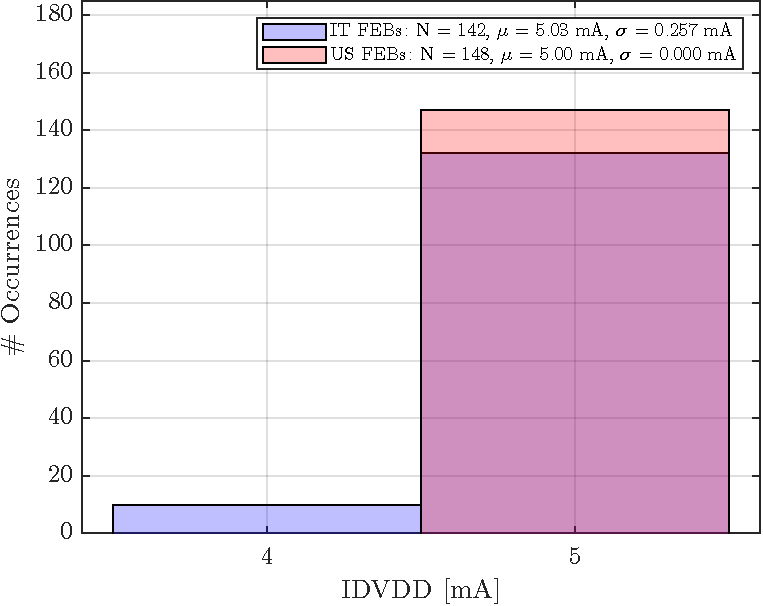
\includegraphics[width=0.477\textwidth]{Images/chap2/results/IDVDD.pdf}\\
    \end{tabular}
    \caption{DVDD values distribution, on the left, and IDVDD values distribution, on the right. Each histogram reports the mean value and standard deviation for both Italian and US productions.}
    \label{figDVDDIDVDD}
\end{figure}

\paragraph{3V3 and I3V3} The distribution of the voltage used as a power supply for calibration, 3V3, and the associated current, I3V3, are shown in \hyperref[fig3V3I3V3]{Figure \ref{fig3V3I3V3}}. It can be seen that the voltage distribution in the case of American production has almost twice the dispersion of Italian production. This phenomenon is attributed to the fact that for 6 FEBs, values greatly different from the expected one are obtained, up to \SI{2.33}{\percent} less. On the other hand, for the Italian production, all measured values are are consistent with the mean, with a standard deviation of \SI{5.00}{\milli\volt}.

\begin{figure}[ht]
    \centering
    \begin{tabular}{cc}
        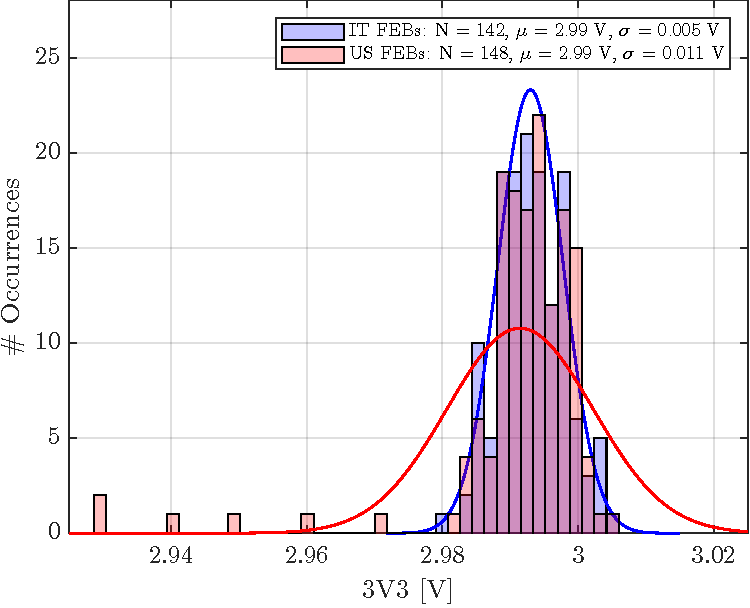
\includegraphics[width=0.467\textwidth]{Images/chap2/results/3V3.pdf} & 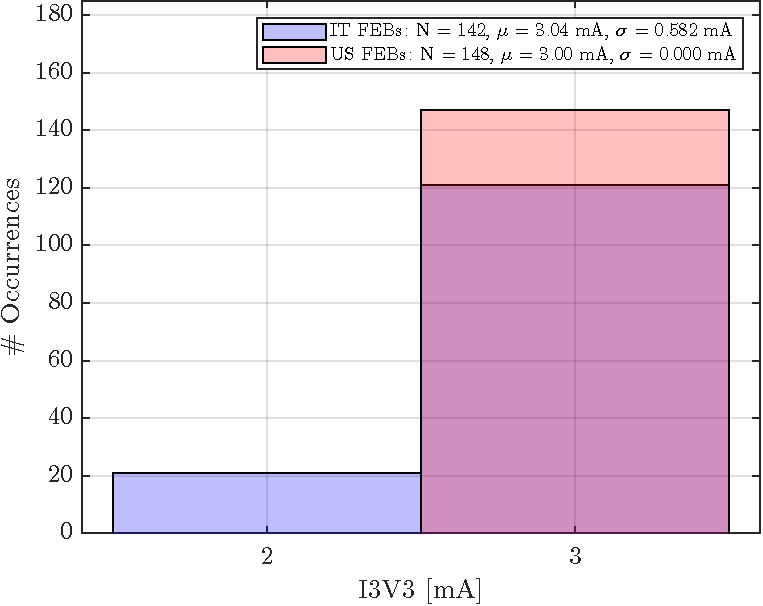
\includegraphics[width=0.477\textwidth]{Images/chap2/results/I3V3.pdf}\\
    \end{tabular}
    \caption{3V3 values distribution on the left and I3V3 values distribution on the right. Each histogram reports the mean value and standard deviation for both Italian and US productions.}
    \label{fig3V3I3V3}
\end{figure}

\begin{figure}[h!]
    \centering
    \begin{tabular}{cc}
        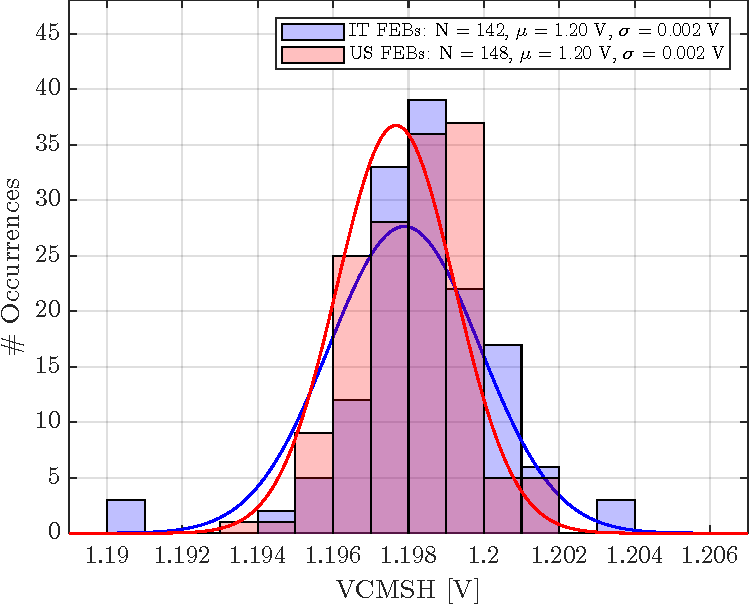
\includegraphics[width=0.475\textwidth]{Images/chap2/results/VCMSH.pdf} & 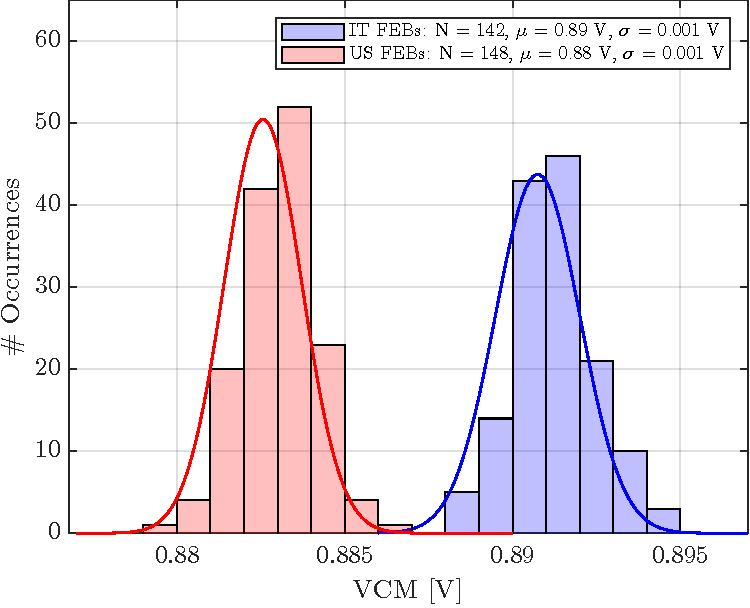
\includegraphics[width=0.475\textwidth]{Images/chap2/results/VCM.pdf}\\
        \multicolumn{2}{c}{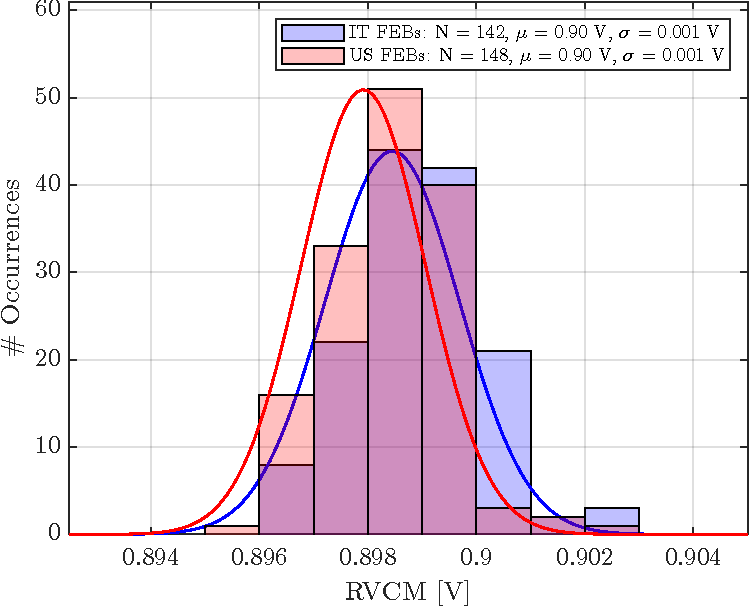
\includegraphics[width=0.475\textwidth]{Images/chap2/results/RVCM.pdf}}
    \end{tabular}
    \caption{Clockwise from left to right: VCMSH, VCM and RVCM values distributions. Each histogram reports the mean value and standard deviation for both Italian and US productions.}
    \label{figVCMSHVCMRVCM}
\end{figure}

\paragraph{VCMSH, VCM and RVCM} \hyperref[figVCMSHVCMRVCM]{Figure \ref{figVCMSHVCMRVCM}} shows the distributions of voltages used as references for the S\&H, shaper and ADC respectively. In the case of VCMSH and RVCM, the average values for both distributions are comparable with the reference value of \SI{1.20}{\volt} and \SI{0.90}{\volt} respectively. In the specific case of the VCM voltage, the Italian and American productions present an average value that differs by approximately \SI{10}{\milli\volt} from each other, while maintaining a comparable standard deviation.

\paragraph{Temperature} The temperature measurements shown in \hyperref[figFEBtemp]{Figure \ref{figFEBtemp}} allows to verify the correct operation of the temperature sensor installed on the front-end board. It can be seen that the average temperature measured on the American-made FEBs is higher than that measured on the Italian-made FEBs. This is purely attributable to the period of the year in which the tests were carried out, that is, summer, therefore an increase in the average measured temperature can be expected. Furthermore, the fact that the tests on the American production were completed within approximately two weeks can be seen in the lower standard deviation, which can be attributed to a smaller fluctuation in ambient temperature. In order to obtain the temperature measurement from the sensor installed on the front-end board (Texas Instruments LMT84), it is first necessary to obtain the output voltage value $V_{T}$, which considering the sensor readout network implemented on the ASIC is evaluated as:

\begin{figure}[h!]
    \centering
    \begin{tabular}{cc}
        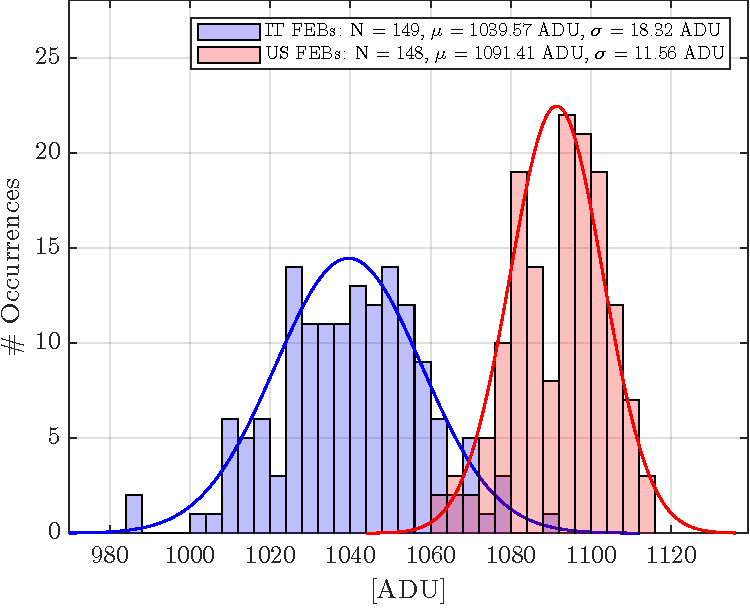
\includegraphics[width=0.475\textwidth]{Images/chap2/results/temperatura_ADC.pdf} & 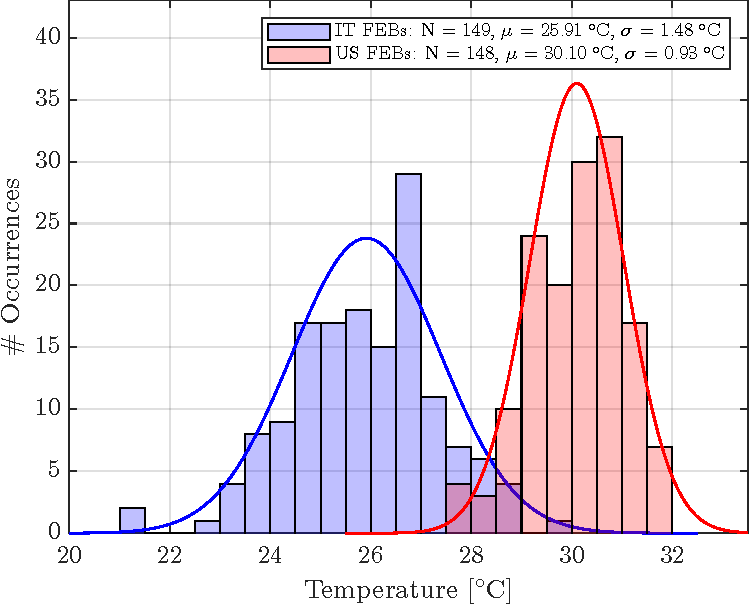
\includegraphics[width=0.475\textwidth]{Images/chap2/results/temperatura_C.pdf}\\
    \end{tabular}
    \caption{Temperature statics for Italian made FEBs: temperature expressed in Analog Digital Units (ADU) on the left and in Celsius (\SI{}{\celsius}) on the right. Each histogram reports the mean value and standard deviation for both Italian and US productions.}
    \label{figFEBtemp}
\end{figure}

% temperature conversion [ADC_code > °C]
% voltage
\begin{equation}
    V_{T} = \SI{900}{\milli\volt} - \frac{(ADC_{code} - 1024) \cdot \SI{1.72}{\milli\volt}}{3.87}.
\end{equation}

\noindent
From this Equation the temperature T can be obtained (expressed in \SI{}{\celsius}):

% temperature
\begin{equation}
    T = \SI{30}{\celsius} + \frac{\SI{5.506}{\frac{\milli\volt}{\celsius}} - \sqrt{(\SI{-5.506}{\frac{\milli\volt}{\celsius}})^2 + 4 \cdot \SI{0.00176}{\frac{\milli\volt}{\celsius^2}} \cdot (\SI{870.6}{\milli\volt} - V_{T})}}{2 \cdot (\SI{-0.00176}{\frac{\milli\volt}{\celsius^2}})}
\end{equation}

\paragraph{Defects detected during visual inspection} \hyperref[figFEBdefects1]{Figure \ref{figFEBdefects1}} shows a comparison of the categories of defects detected on Italian and American-made FEBs during visual inspection, while \hyperref[figFEBdefects2]{Figure \ref{figFEBdefects2}} shows the percentage of FEBs with and without defects detected for both productions. It can be seen that although the percentage of defects detected differs significantly between the two productions, the overall percentage of defect-free front-end boards is comparable.

\begin{figure}[h!]
    \centering
    \begin{tabular}{cc}
        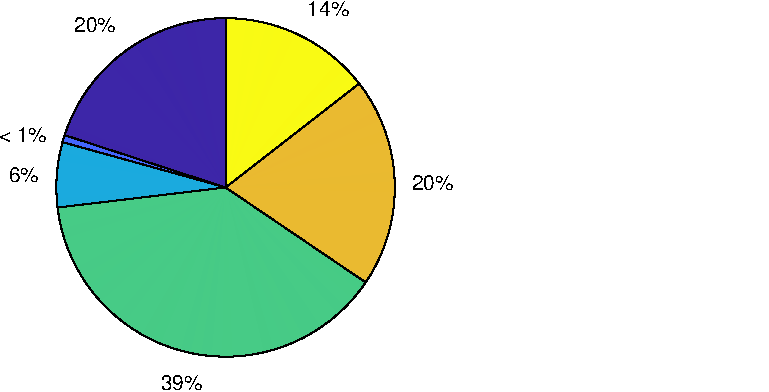
\includegraphics[width=0.35\textwidth]{Images/chap2/results/defects_category_IT.pdf} & 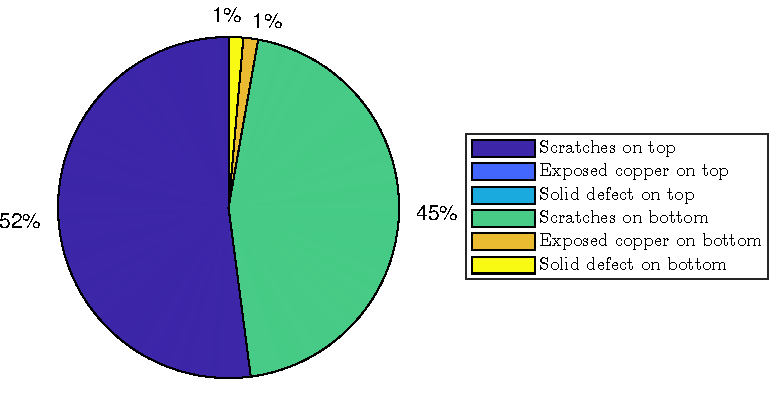
\includegraphics[width=0.58\textwidth]{Images/chap2/results/defects_category_US.pdf}\\
    \end{tabular}
    \caption{Defects found during visual inspection on Italian made FEBs (on the left) and on US-made ones (on the right).}
    \label{figFEBdefects1}
\end{figure}

\begin{figure}[h!]
    \centering
    \begin{tabular}{c p{8.6cm}}
        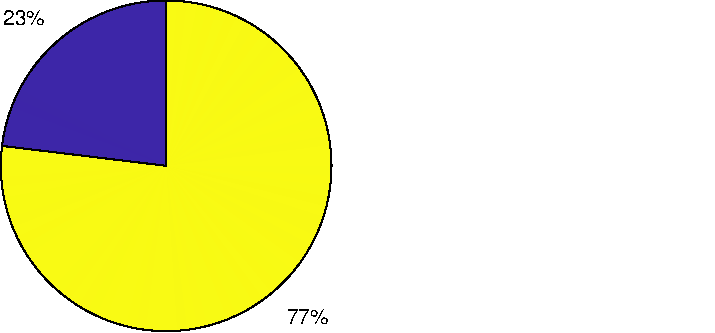
\includegraphics[width=0.285\textwidth]{Images/chap2/results/defects_number_IT.pdf} & 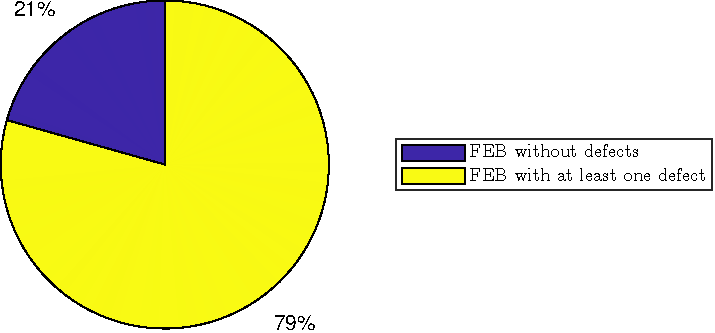
\includegraphics[width=0.6\textwidth]{Images/chap2/results/defects_number_US.pdf}\\
    \end{tabular}
    \caption{Percentage of FEB without any noticeable visual defects for the Italian production (on the left) and for the US production (on the right).}
    \label{figFEBdefects2}
\end{figure}

\paragraph{Pedestal dispersion} This paragraph reports the results of the pedestal measurement used to evaluate the electronic noise of each channel in order to identify the most problematic ones, which could adversely affect the correct measurement of incident charges. The plot in \hyperref[figFEBpedestal]{Figure \ref{figFEBpedestal}} represents the distribution of pedestal dispersion evaluated on the FEBs of Italian and US production. It is easy to deduce how the use of the metal box induces a reduction in pedestal dispersion, which in US-made FEBs is reduced by about \SI{83}{\percent} in mean value and \SI{74}{\percent} in terms of standard deviation compared to Italian-made ones.

\begin{figure}[h!]
    \centering
    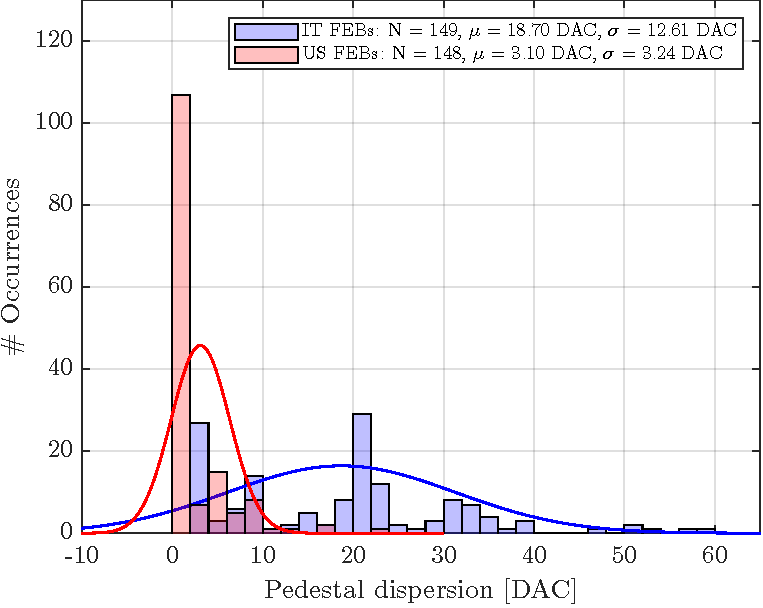
\includegraphics[width=0.55\textwidth]{Images/chap2/results/ped_disp.pdf}
    \caption{Pedestal dispersion distribution. The histogram reports the mean value and standard deviation for both Italian and US productions.}
    \label{figFEBpedestal}
\end{figure}

\paragraph{Threshold dispersion} \hyperref[figFEBthreshold]{Figure \ref{figFEBthreshold}} presents the distributions of threshold dispersion before fine threshold optimisation (on the left) and after (on the right). It can be seen that, after optimisation using the 3-bit DAC, both distributions from Italian and US production, have a reduced dispersion as well as a compatible mean and standard deviation since the minimisation process focuses on obtaining a threshold voltage value consistent across all the modules integrated in the tracker. Fine threshold tuning via the aforementioned 3-bit DAC in fact allows the threshold voltage to be optimised directly on the individual channel, thus making it possible to bring the threshold value of the channel closer to the global threshold value. This is made necessary by the fact that, due to variations in the manufacturing process of the transistors constituting the channel circuit blocks, each channel has a threshold value slightly different from one another and not necessarily equal to the set global threshold value. This method therefore allows one to act at a "fine" level in order to reduce the overall threshold dispersion over all 32 channels. 

\par
The result of applying this method is immediately visible by comparing the standard deviations of the distributions shown in \hyperref[figFEBthreshold]{Figure \ref{figFEBthreshold}}, which highlights how the dispersion value after optimisation is on average reduced by half on both productions.

\begin{figure}[h!]
    \centering
    \begin{tabular}{cc}
        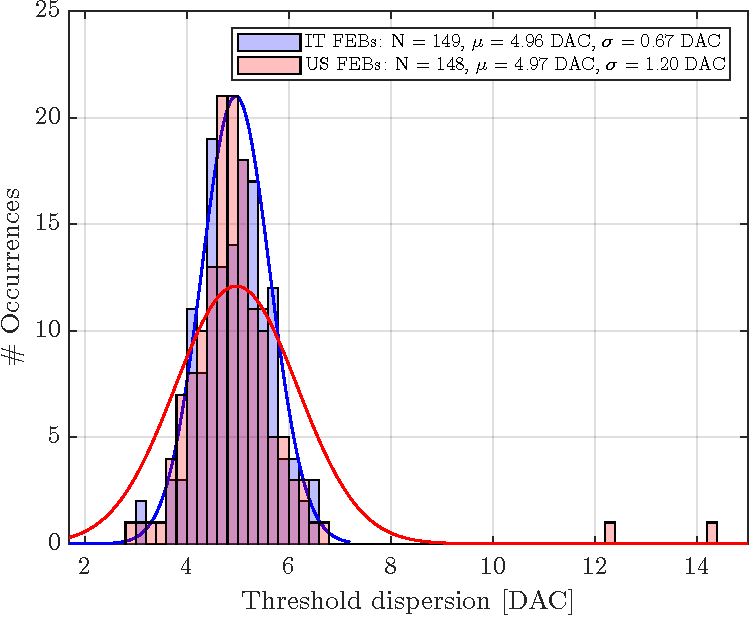
\includegraphics[width=0.475\textwidth]{Images/chap2/results/thrdisp_bef.pdf} & 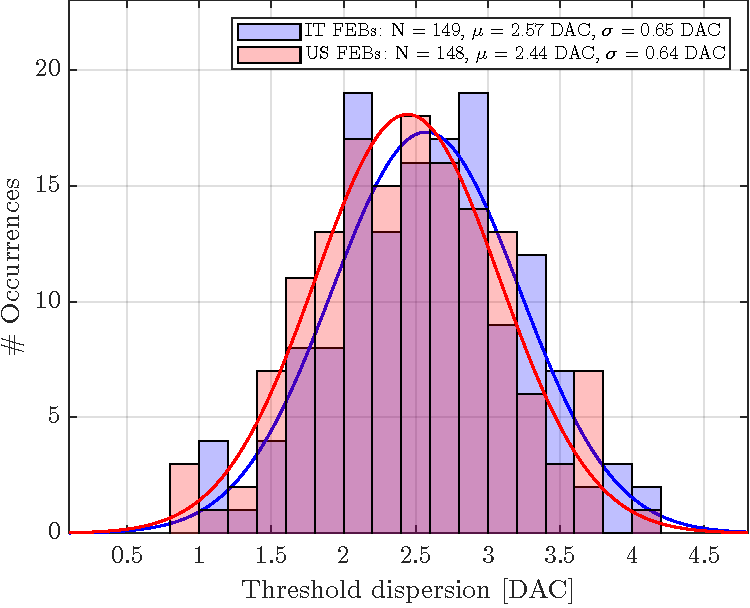
\includegraphics[width=0.475\textwidth]{Images/chap2/results/thrdisp_aft.pdf}\\
    \end{tabular}
    \caption{Threshold dispersion values distribution before fine threshold optimisation (on the left) and after (on the right). Each histogram reports the mean value and standard deviation for both Italian and US productions.}
    \label{figFEBthreshold}
\end{figure}

\paragraph{Noise} The noise measurements carried out on 135 of the 150 American-made FEBs are shown in \hyperref[figFEBNoise]{Figure \ref{figFEBNoise}} for channels No. 0, 7, 15, 16, 23, 31. In particular, the displayed measurements were carried out by placing the front-end board under test inside a metal box in order to shield it from the electromagnetic interferences present in the test environment. This made it possible to obtain noise measurements, in the form of ENC, that could effectively reflect the real noise performance of the boards, free of alterations due to the surrounding environment. The remaining FEBs, including those of Italian manufacture, were tested without any shielding and demonstrated ENC values even in the hundreds of \SI{}{\kilo\electronvolt} range.

\begin{figure}[h!]
    \centering
    \begin{tabular}{cc}
        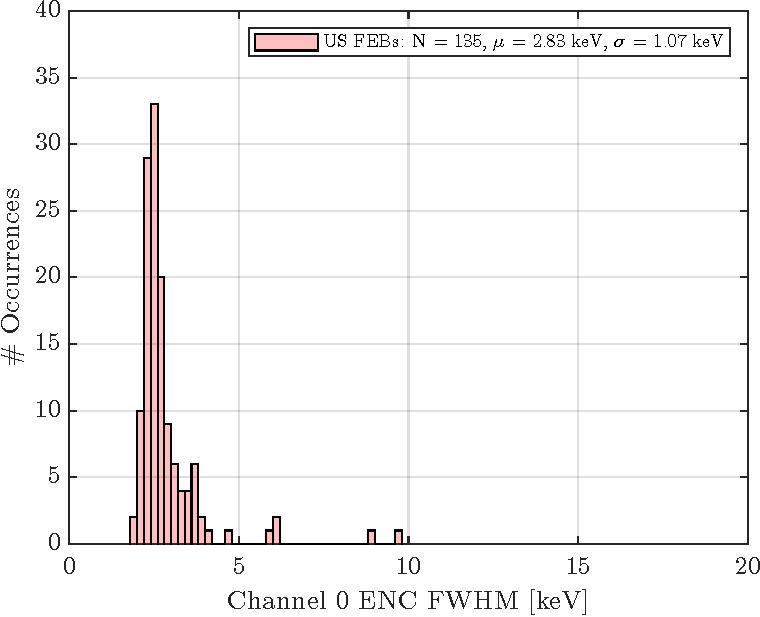
\includegraphics[width=0.475\textwidth]{Images/chap2/results/ENC_0.pdf} & 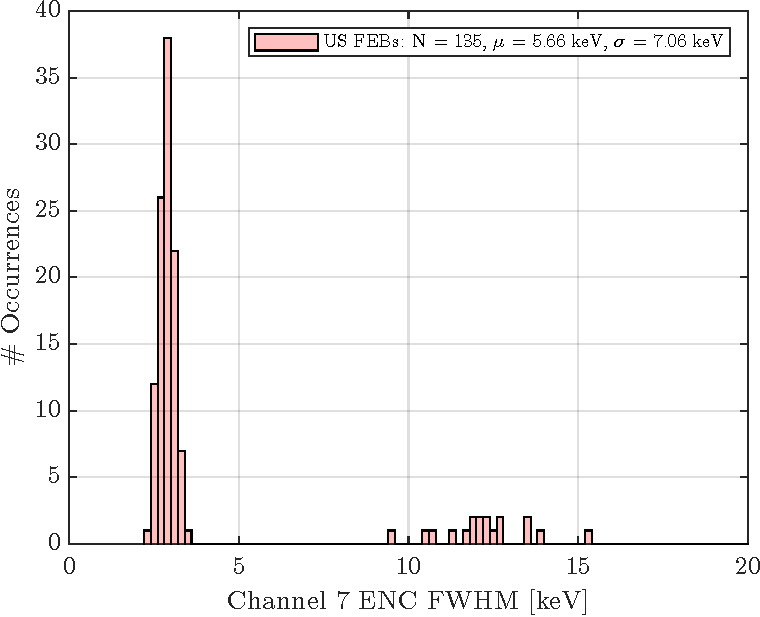
\includegraphics[width=0.475\textwidth]{Images/chap2/results/ENC_7.pdf}\\
        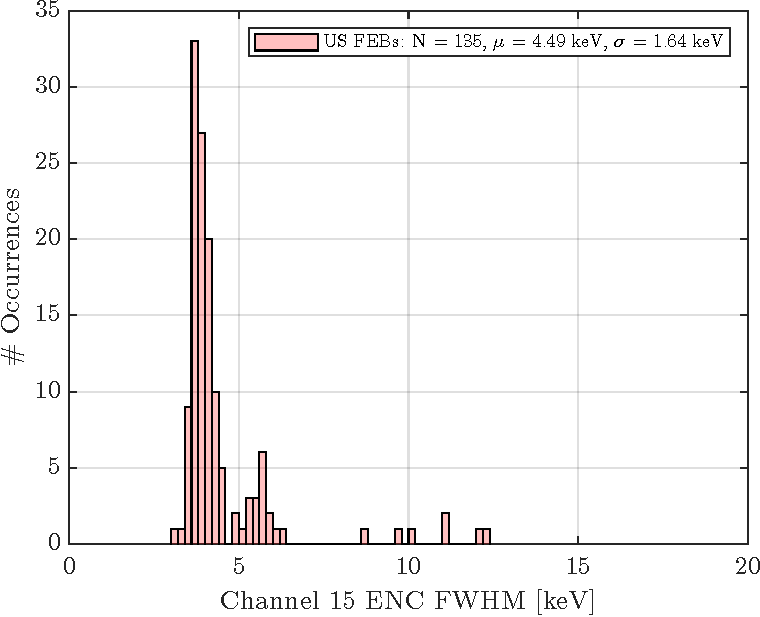
\includegraphics[width=0.475\textwidth]{Images/chap2/results/ENC_15.pdf} & 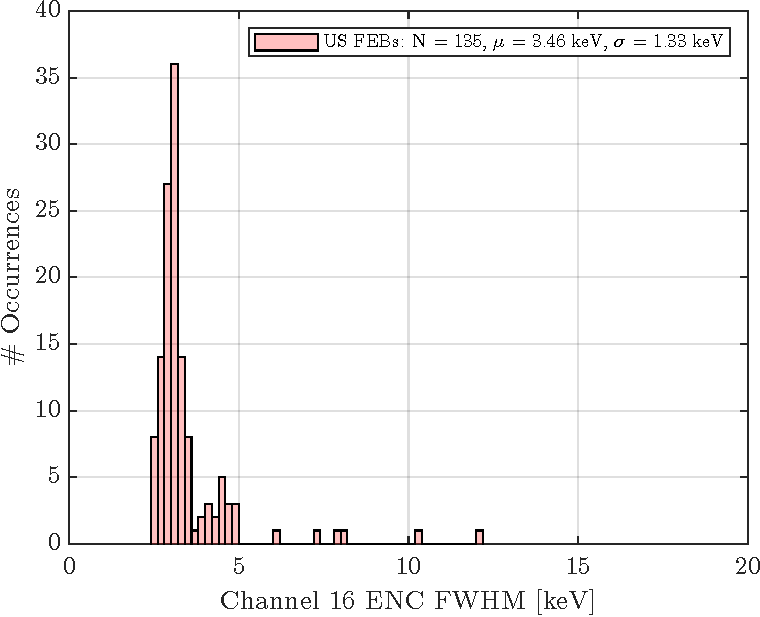
\includegraphics[width=0.475\textwidth]{Images/chap2/results/ENC_16.pdf}\\
        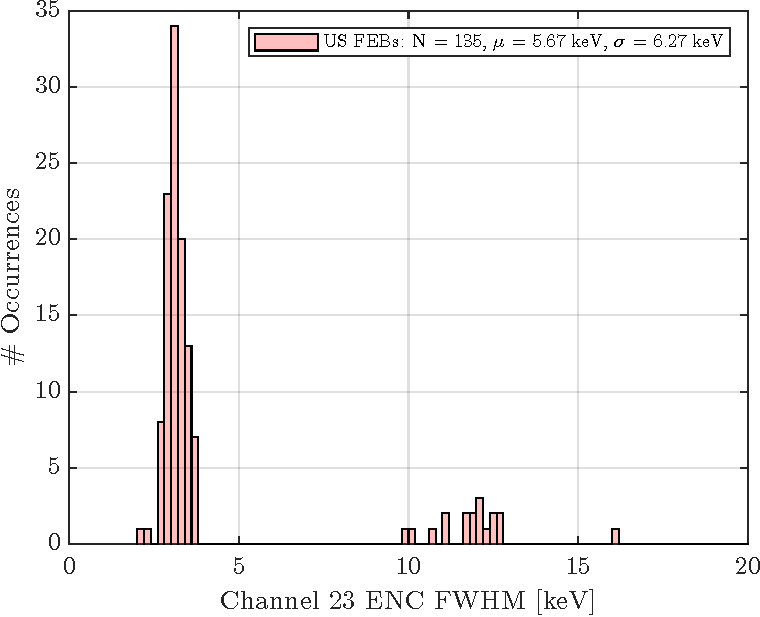
\includegraphics[width=0.475\textwidth]{Images/chap2/results/ENC_23.pdf} & 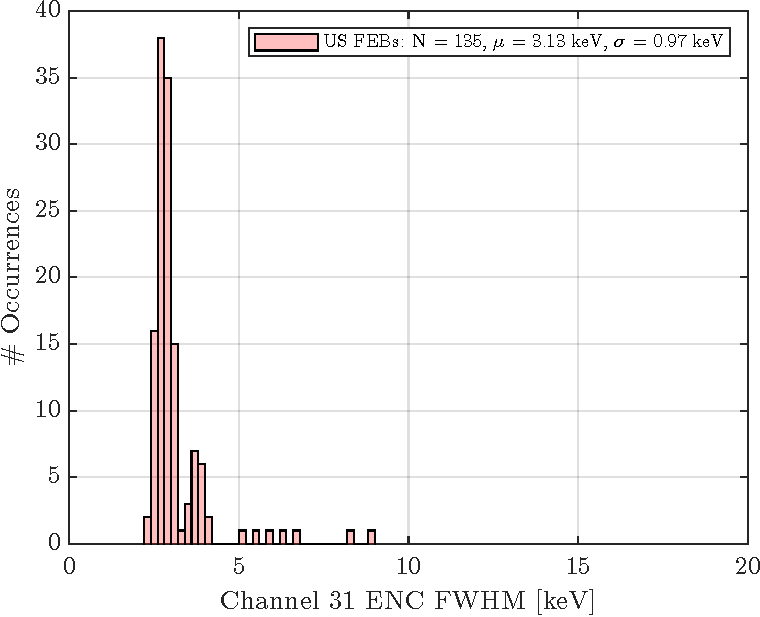
\includegraphics[width=0.475\textwidth]{Images/chap2/results/ENC_31.pdf}\\
    \end{tabular}
    \caption{Statistical distributions of measured ENC FWHM for a limited set of boards belonging to the US production. Each histogram also reports the distribution mean value and standard deviation.}
    \label{figFEBNoise}
\end{figure}


%-------------------------------------------------------------------------------
%   Dummy-1 front-end board
%-------------------------------------------------------------------------------

\section{Dummy-1 front-end board} \label{sec22}

The Dummy board type 1, also known as \textit{Dummy-1}, is a not populated board that will be used in the first launch of the experiment, scheduled for the end of 2023, in order to replace the missing FEBs in some of the detector layers, as these are currently in a smaller number than required to fill all the tracker slots.

The validation tests of the Dummy-1 front-end boards has been performed at ambient temperature after having soldered only a couple of resistors emulating the analog power consumption of the FEB. Specifically, two \SI{40}{\ohm} resistors and a \SI{4.7}{\micro\farad} capacitor 0805 SMD have been installed on the board, along with a short piece of wire ($\approx\SI{1}{\cm}$ in length) in order to connect the newly installed components to the analog voltage supply line, as shown in \hyperref[figDummySoldering]{Figure \ref{figDummySoldering}}. 

\begin{figure}[h!]
    \centering
    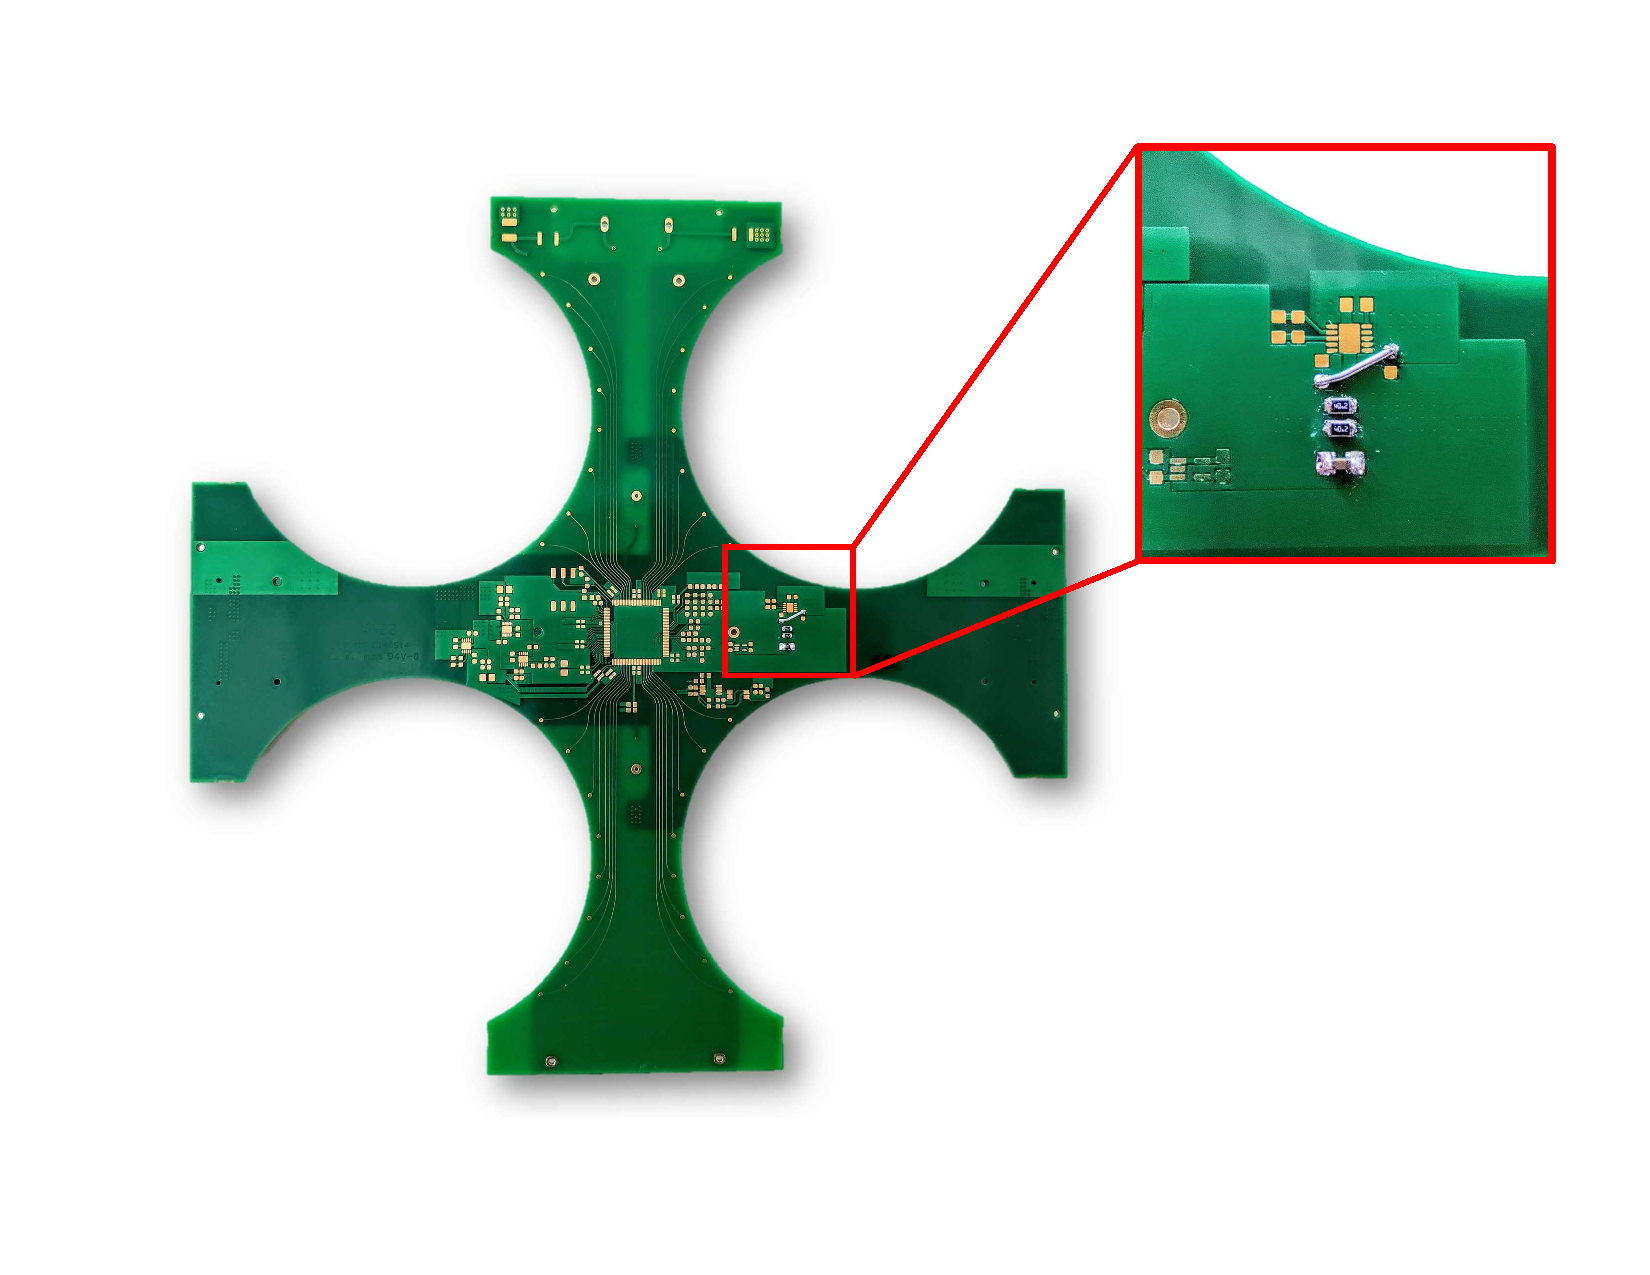
\includegraphics[width=0.95\textwidth]{Images/chap2/dummy_image.pdf}
    \caption{Dummy-1 front-end board with a detailed view of the soldered components.}
    \label{figDummySoldering}
\end{figure}

This configuration was chosen as the one better suited to emulate the thermal behaviour of the active components installed on a fully populated FEB. Initial trials were based on a single \SI{20}{\ohm} 0805 SMD resistor directly connected to the AVDD supply voltage, but this configuration was soon discarded as the power dissipated by the resistor was very near to its \SI{0.5}{\watt} maximum power rating. In fact, the current flowing through the resistor is evaluated as

\begin{equation}
    I_{R} = \frac{\SI{2.8}{\volt}}{\SI{20}{\ohm}} = \SI{0.14}{\ampere} = \SI{140}{\milli\ampere} 
\end{equation}

\noindent
therefore the power dissipated by the resistor is

\begin{equation}
    P_{R} = \SI{2.8}{\volt} \cdot \SI{0.14}{\ampere} = \SI{0.392}{\watt} 
\end{equation}

\noindent
which confirms the aforementioned. A common rule of thumb requires the power rating to be at least twice the nominal dissipated power, therefore employing two \SI{40}{\ohm} resistors in parallel allowed the power dissipated on each resistor to be half of the total dissipated power

\begin{equation}
    P_{R} = \SI{2.8}{\volt} \cdot \frac{\SI{0.14}{\ampere}}{2} = \SI{0.196}{\watt}
\end{equation}

\noindent
thus ensuring compliance to the aforementioned rule of thumb. \hyperref[figDummyThermal]{Figure \ref{figDummyThermal}} shows the thermal image for the configuration with a single resistor (on the left) and with two resistors (on the right). In both cases, the analog supply voltage (AVDD) was set to \SI{2.8}{\volt}, as a worst case scenario. It can be seen the temperature difference between the two configurations is of approximately \SI{9.8}{\celsius} for the same dissipated power.

\begin{figure}[h!]
    \centering
    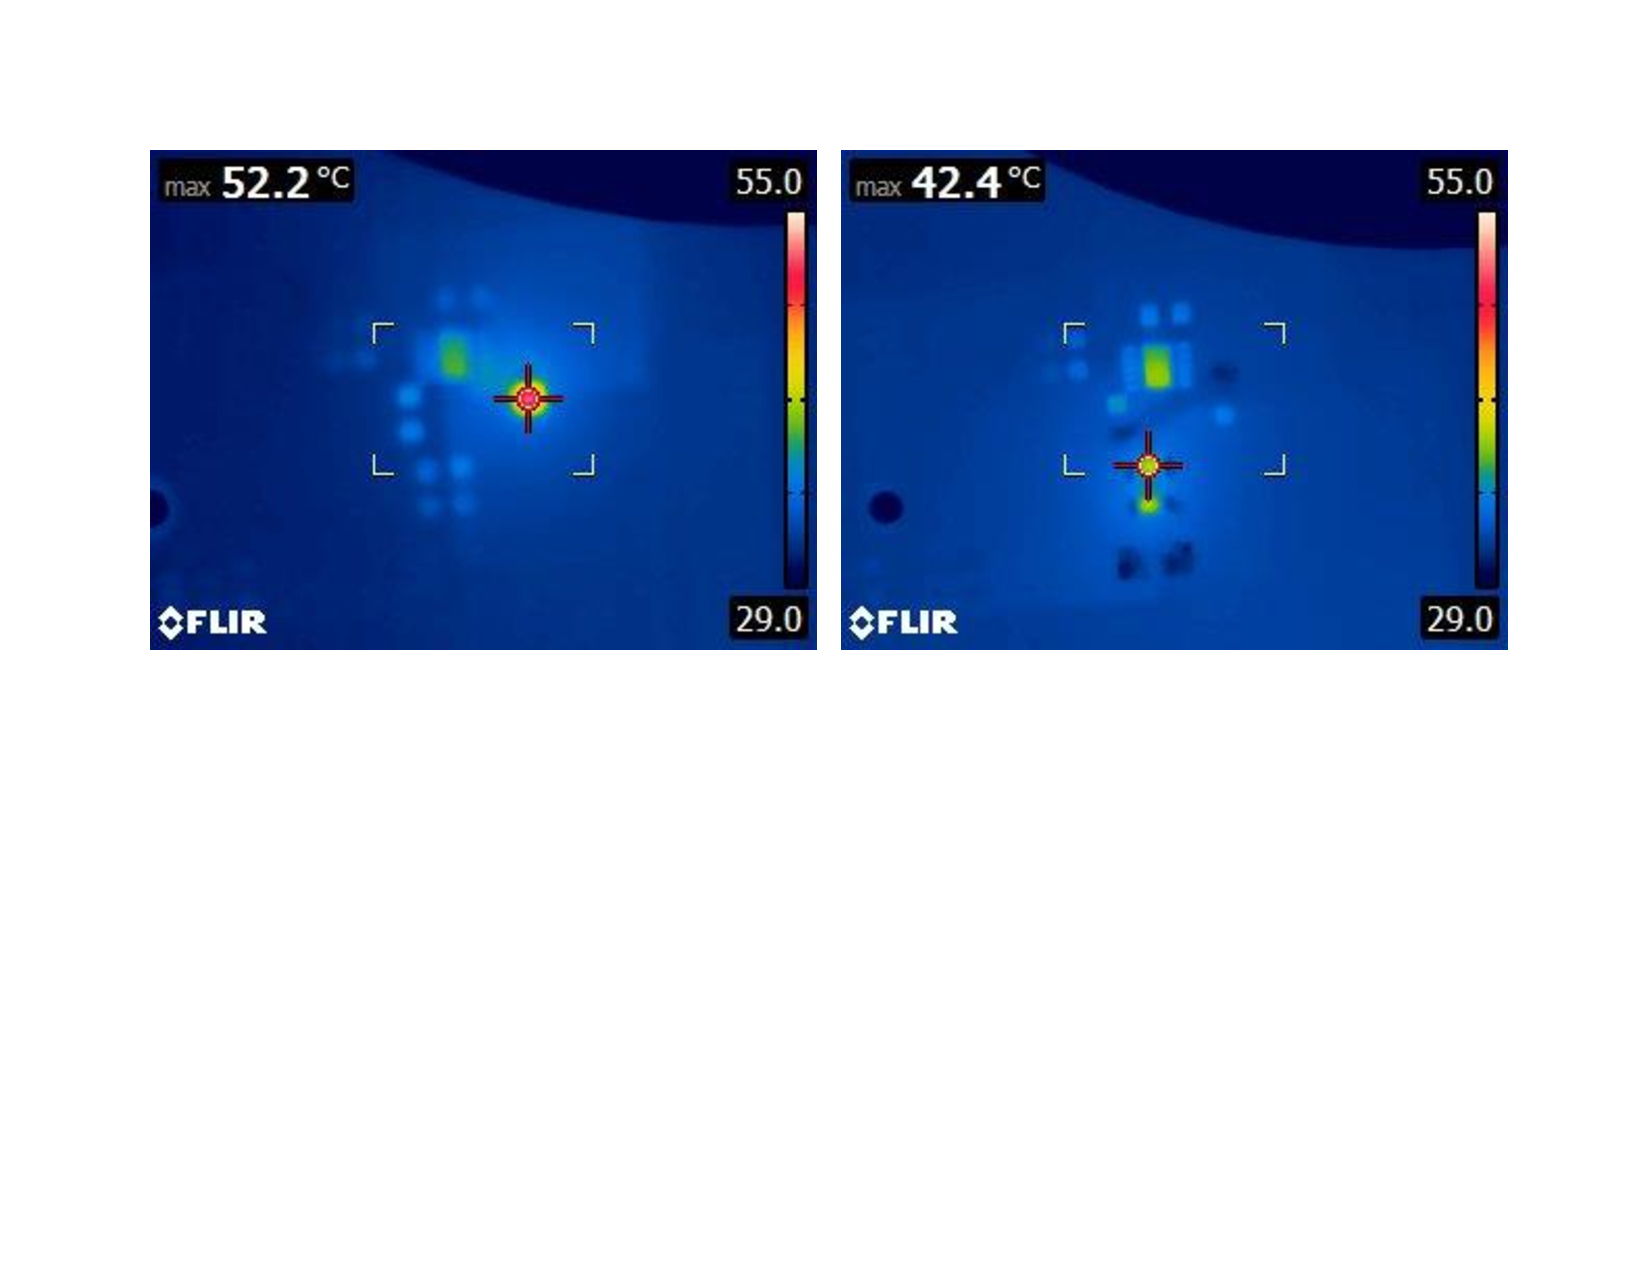
\includegraphics[width=0.8\textwidth]{Images/chap2/DUMMY_bef_aft.pdf}
    \caption{Thermal performance of Dummy-1 boards: on the left the configuration with a single \SI{20}{\ohm} resistor, on the right the configuration with two \SI{40}{\ohm} resistors in parallel.}
    \label{figDummyThermal}
\end{figure}

\par
\noindent
Tests carried out on the Dummy-1 FEBs have the purpose of:

\begin{itemize}
    \itemsep0em 
    \item Verify that the board is able to emulate the proper power dissipation.
    \item Verify that, once placed in series with other FEBs, it is able to properly propagate both bias voltages and digital signals to the subsequent boards.
\end{itemize}

%-------------------------------------------------------------------------------

\subsection{Visual inspection}
A manual visual inspection has been performed for each Dummy-1 sample by looking over the board either with the naked eye or through magnification. Visual inspection has been applied before and after the thermal cycle. The purpose of this activity is to look for missing or bad-soldered ERNI connectors and defects (pits, dents, scratches, pinholes and other defects on printing traces and pads). If no or negligible defects were found, \texttt{[YES]} was reported in the \textit{Visual Inspection} field of the test report module. If a missing or bad-soldered component was found, the board was rejected since it is not possible to manually solder the ERNI connectors.

%-------------------------------------------------------------------------------

\subsection{Thermal test} \label{subsection-thermal}
The boards underwent one thermal cycle in a climate chamber (model ACS DY110) in order to ensure that the board and the components installed on it are not deformed or damaged under the operating temperature conditions of the experiment, thus also verifying the correct soldering of the components on the board. The performed thermal cycle has the following characteristics:

\begin{itemize}
    \itemsep0em 
    \item Minimum temperature (\texttt{$T_{min}$}): \SI{-40}{\celsius}.
    \item Maximum temperature (\texttt{$T_{max}$}): +\SI{60}{\celsius}.
    \item Time spent at $T_{min}$ and $T_{max}$: 20 minutes.
    \item Heating and cooling rate: Maximum \SI{4}{\celsius/minute}.
\end{itemize}

\noindent
If, after the thermal cycle, the PCB did not show any type of defect, \texttt{[YES]} was reported in the \textit{Thermal Cycle} field of the test report module. A plot of the temperature in the climate chamber during thermal test can be found in \hyperref[figDUMMYtest]{Figure \ref{figDUMMYtemp}}, where the \SI{60}{\celsius} and \SI{-40}{\celsius} intervals are visible. It can be also noted that the boards underwent a further 20 minutes at controlled ambient temperature ($\approx\SI{25}{\celsius}$) after the thermal cycle was completed in order to avoid any thermal shocks or damages coming from a sudden change in temperature.

\begin{figure}[h!]
    \centering
    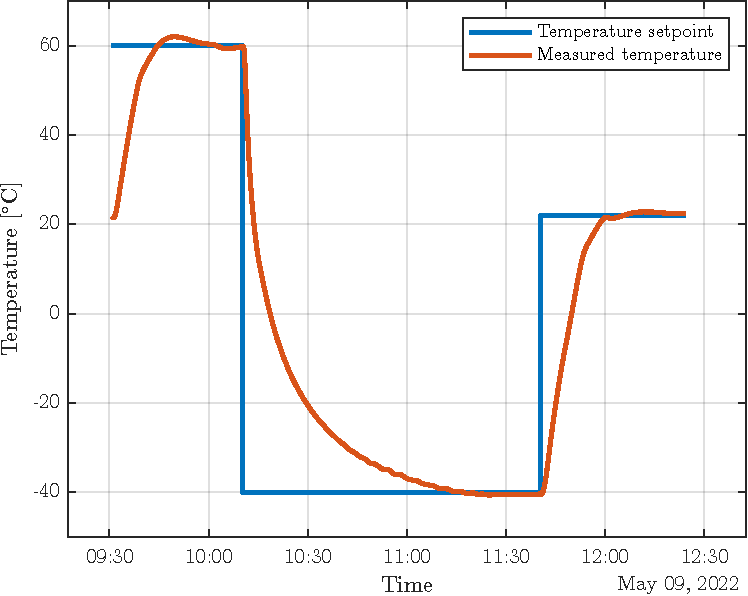
\includegraphics[width=0.6\textwidth]{Images/chap2/chamber_temperature.pdf}
    \caption{Environmental chamber temperature trend during thermal test (in orange) compared to the set-point (in blue).}
    \label{figDUMMYtemp}
\end{figure}

After the thermal cycle, the boards have been left biased for at least 10 minutes. If no damage occurred to the resistors, the test is considered as passed. Moreover, a thermal picture of the resistor has been taken (with a FLIR ETS320 non-contact thermal measurement system), like the one shown in \hyperref[figDummyThermal]{Figure \ref{figDummyThermal}}.

%-------------------------------------------------------------------------------

\subsection{Power test}
In this test a nominal voltage of \SI{2.8}{\volt} was applied to the board. The current IAVDD absorbed and the voltage APDD of the dummy resistor have been measured and reported on the test report together with the computed power consumption PAVDD. For these measurements, the pass/fail criterion is not obvious, so the typical measurement value has been determined iteratively by analysing the scans of a larger number of boards.

%-------------------------------------------------------------------------------

\subsection{Bias and Digital}
The purpose of this test is to validate the soldering of the input and output ERNI connectors. The board under test has been placed in series with a fully populated FEB as shown in \hyperref[figFEBtest2]{Figure \ref{figFEBtest2}} and a configuration test was run on the FEB. If it responded correctly, it means that ERNI connectors on the Dummy-1 board are properly soldered and \texttt{[YES]} has been reported in the \textit{Communication test} field of the test report.

\par
As done for the front-end boards, a test report is generated, whose first page is shown in \hyperref[figDUMMYreport]{Figure \ref{figDUMMYreport}}. In the case of the Dummy-1 front-end boards, a single multi-page document has been created, having the structure described in \hyperref[tabDUMMYstruct]{Table \ref{tabDUMMYstruct}}.

\begin{table}[h!]
    \centering
    \def\arraystretch{1.3}
    \resizebox{0.95\columnwidth}{!}{
        \begin{tabular}{|c|c|c|c|c|c|c|} 
            \hline
            $\bm{\#}$ & \textbf{Board ID} & \makecell{\textbf{Thermal}\T \\ \textbf{cycling}\B} & \makecell{\textbf{Visual}\T \\ \textbf{inspection}\B} & \makecell{\textbf{Communication}\T \\ \textbf{test}\B} & \textbf{IAVDD [\SI{}{\milli\ampere}}]\T\B & \textbf{PAVDD [\SI{}{\milli\watt}}]\T\B \\ 
            \hline
            \texttt{1} & \texttt{D00} & \textcolor{ForestGreen}{\texttt{Yes}}/\textcolor{red}{\texttt{No}} & \textcolor{ForestGreen}{\texttt{Yes}}/\textcolor{red}{\texttt{No}} & \textcolor{ForestGreen}{\texttt{Yes}}/\textcolor{red}{\texttt{No}} & \texttt{000.0} & \texttt{000.00}\T\B \\ \hline 
        \end{tabular}
    }
    \caption{Structure of the entry for the Dummy-1 front-end boards test report.}
    \label{tabDUMMYstruct}
\end{table}

%-------------------------------------------------------------------------------

\subsection{Test results}
This Section reports the results of current (IAVDD) and power (PAVDD) measurements taken on all the 62 Dummy-1 front-end boards. The power value was obtained by multiplying the current value by the resistance value obtained from the parallel of the two installed resistors ($R_{tot} = \SI{20}{\ohm}$). \hyperref[figDUMMYresults]{Figure \ref{figDUMMYresults}} shows the distributions of current values on the left and power values on the right.

\begin{figure}[h!]
    \centering
    \begin{tabular}{cc}
        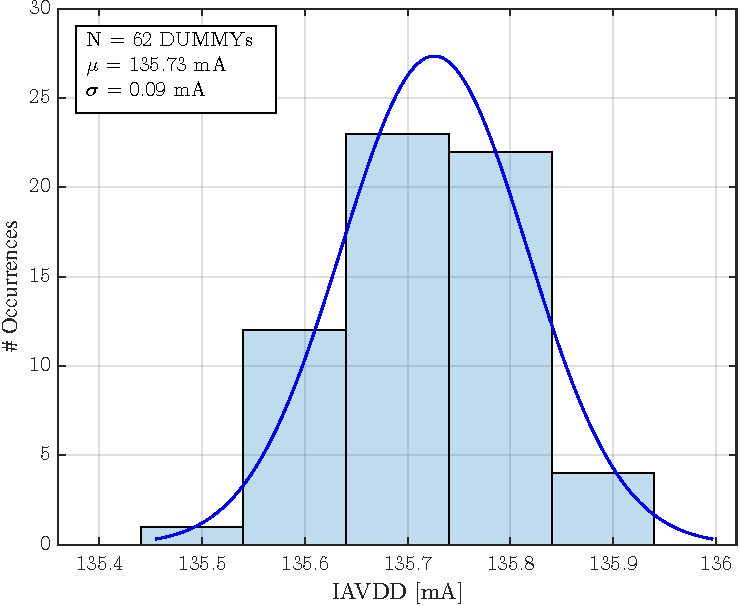
\includegraphics[width=0.475\textwidth]{Images/chap2/results/dummy/AIDD.pdf} & 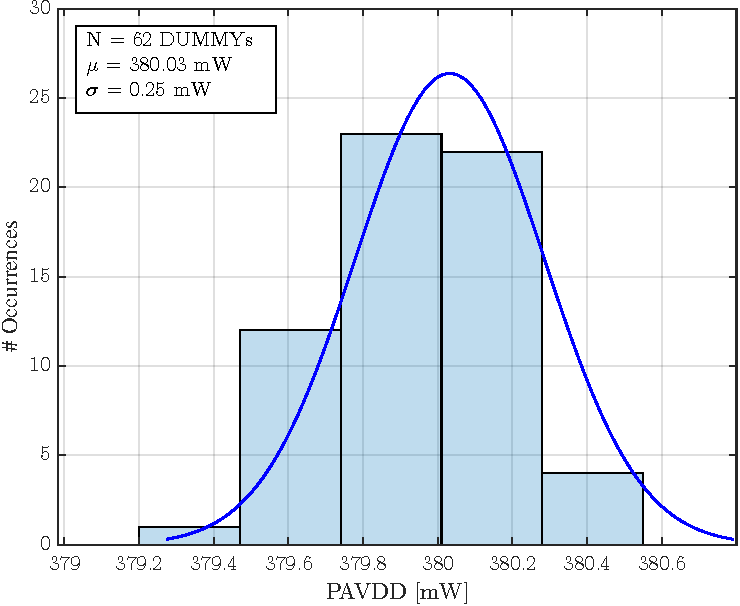
\includegraphics[width=0.475\textwidth]{Images/chap2/results/dummy/APDD.pdf}\\
    \end{tabular}
    \caption{IAVDD values distribution on the left and PAVDD values distribution on the right. Both plots also provide the mean value and standard deviation of the respective distributions.}
    \label{figDUMMYresults}
\end{figure}


%-------------------------------------------------------------------------------
%   Flex-Rigid Board
%-------------------------------------------------------------------------------

\section{Flex-Rigid Board} \label{flexrigids}

Flex-rigid boards are intended to connect one front-end board with the next in the chain. They are by design flexible and allow digital signals and low power voltage supplies to be transported from one module to the next. The flexibility is given both by the material they are made of, polyamide, and by the presence of ground networks instead of rigid ground planes. The dielectric used in these boards is FR4 and they consist of 7 layers for the rigid zone, at the extremes, where the connectors are located, and 3 for the flexible interconnection zone. \hyperref[figDflexrigidPIC]{Figure \ref{figDflexrigidPIC}} presents on the left a picture of a flex-rigid board next to a photograph in which the flex-rigid board is used to connect two front-end boards, where the flexibility of the flex-rigid board can be appreciated.

\subsection{Visual inspection}
A manual visual inspection has been performed for each sample by looking over the board either with the naked eye or through magnification. Visual inspection is applied before and after the thermal cycle. The purpose of this activity was to look for missing or bad-soldered ERNI connectors and defects (pits, dents, scratches, pinholes and other defects on printing traces and pads). If no or negligible defects were found, \texttt{[YES]} has been reported in the \textit{Visual Inspection} field of the test report. If a missing or bad-soldered component was found, the board is rejected since it is not possible to manually solder the ERNI connectors.

\subsection{Thermal cycle}
The flex-rigid boards underwent one thermal cycle in a climate chamber (model ACS DY110). Thermal cycle has the same characteristics described in \hyperref[subsection-thermal]{section \ref{subsection-thermal}}. For flex-rigid boards that underwent thermal cycle and did not show any type of defect, \texttt{[YES]} has been reported in the \textit{Thermal Cycle} field of the test report.

\subsection{Communication test}
The purpose of this test is to validate the soldering of the two ERNI connectors. The board under test was placed in series with two fully populated FEBs as shown in \hyperref[figFEBtest2]{Figure \ref{figFEBtest2}} and a configuration test was run on the second board in the chain. If it responded correctly, it means that ERNI connectors on the Flex-rigid board are properly soldered and \texttt{[YES]} has been reported in the \textit{Communication test} field of the test report. \\

\begin{figure}[h!]
    \centering
    \begin{tabular}{cc}
        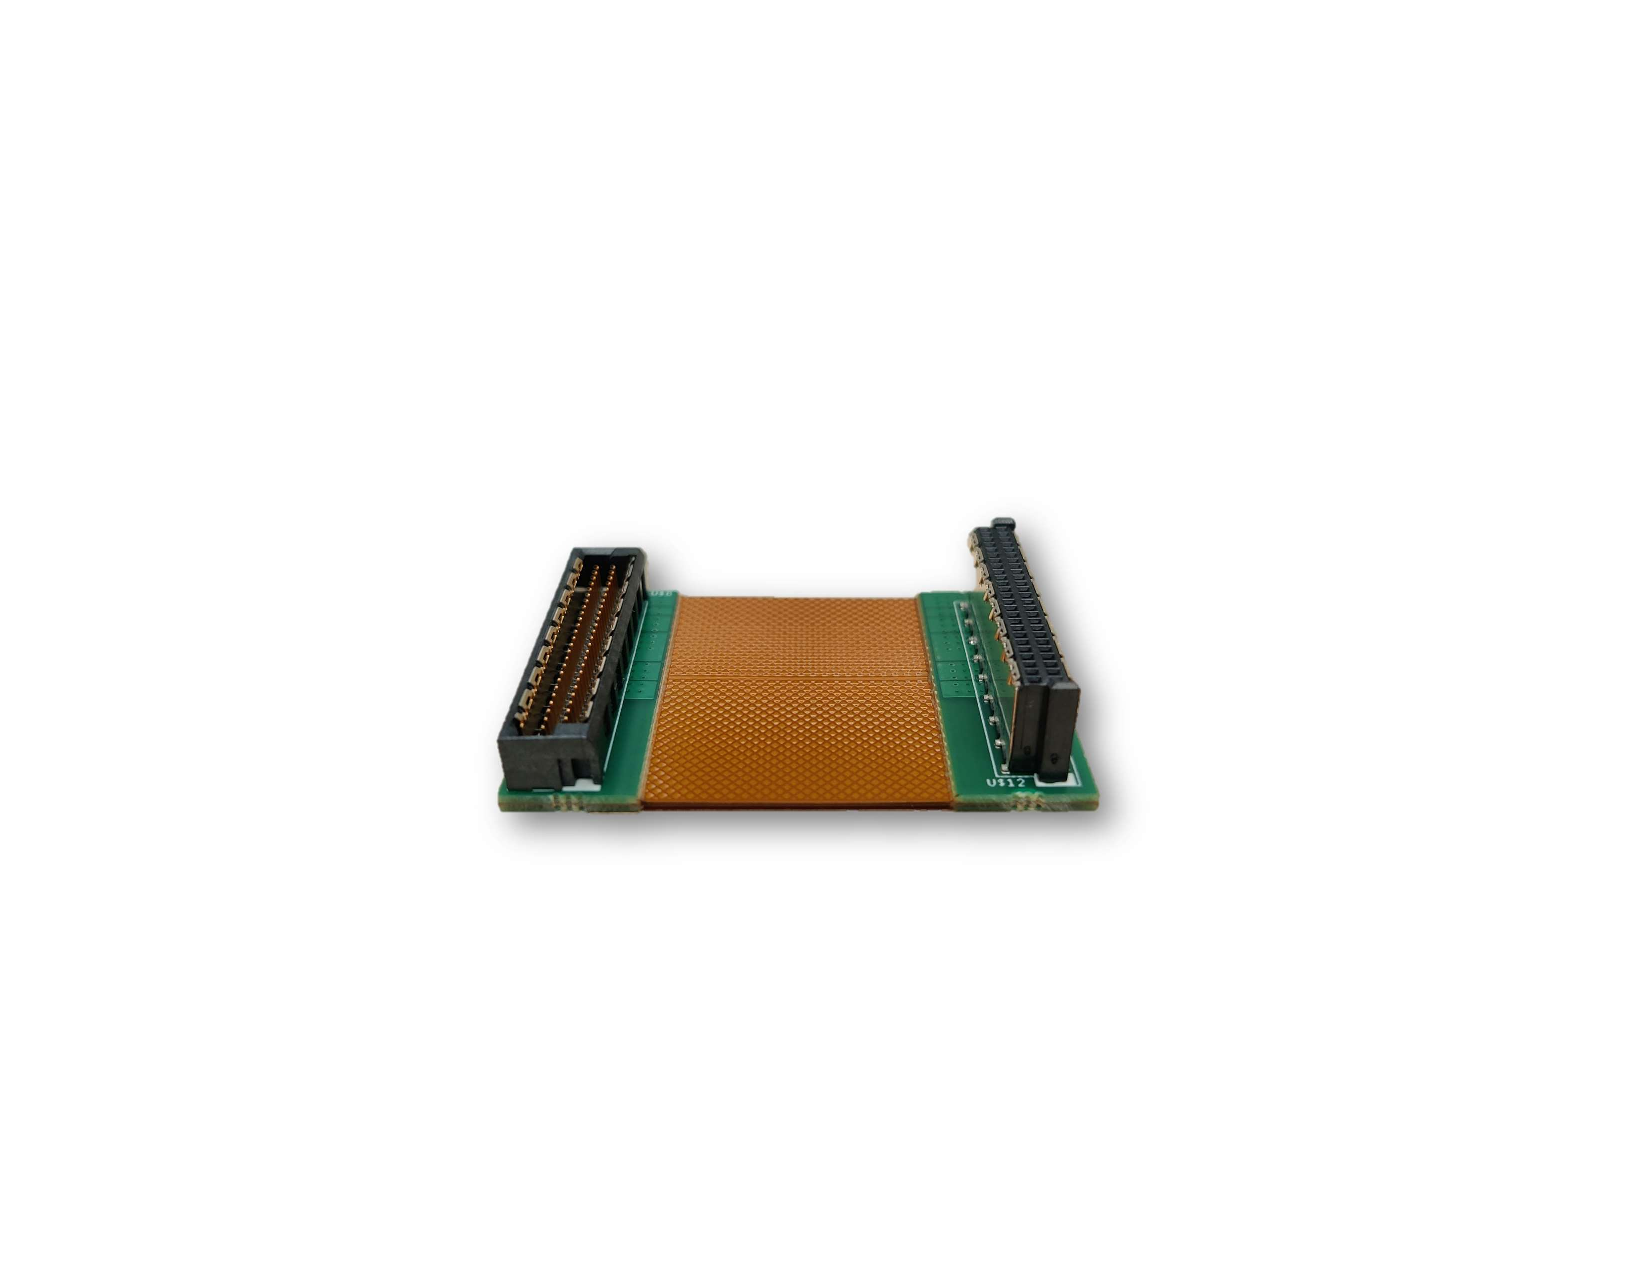
\includegraphics[width=0.38\textwidth]{Images/chap2/flex_rigid_pic.pdf} & 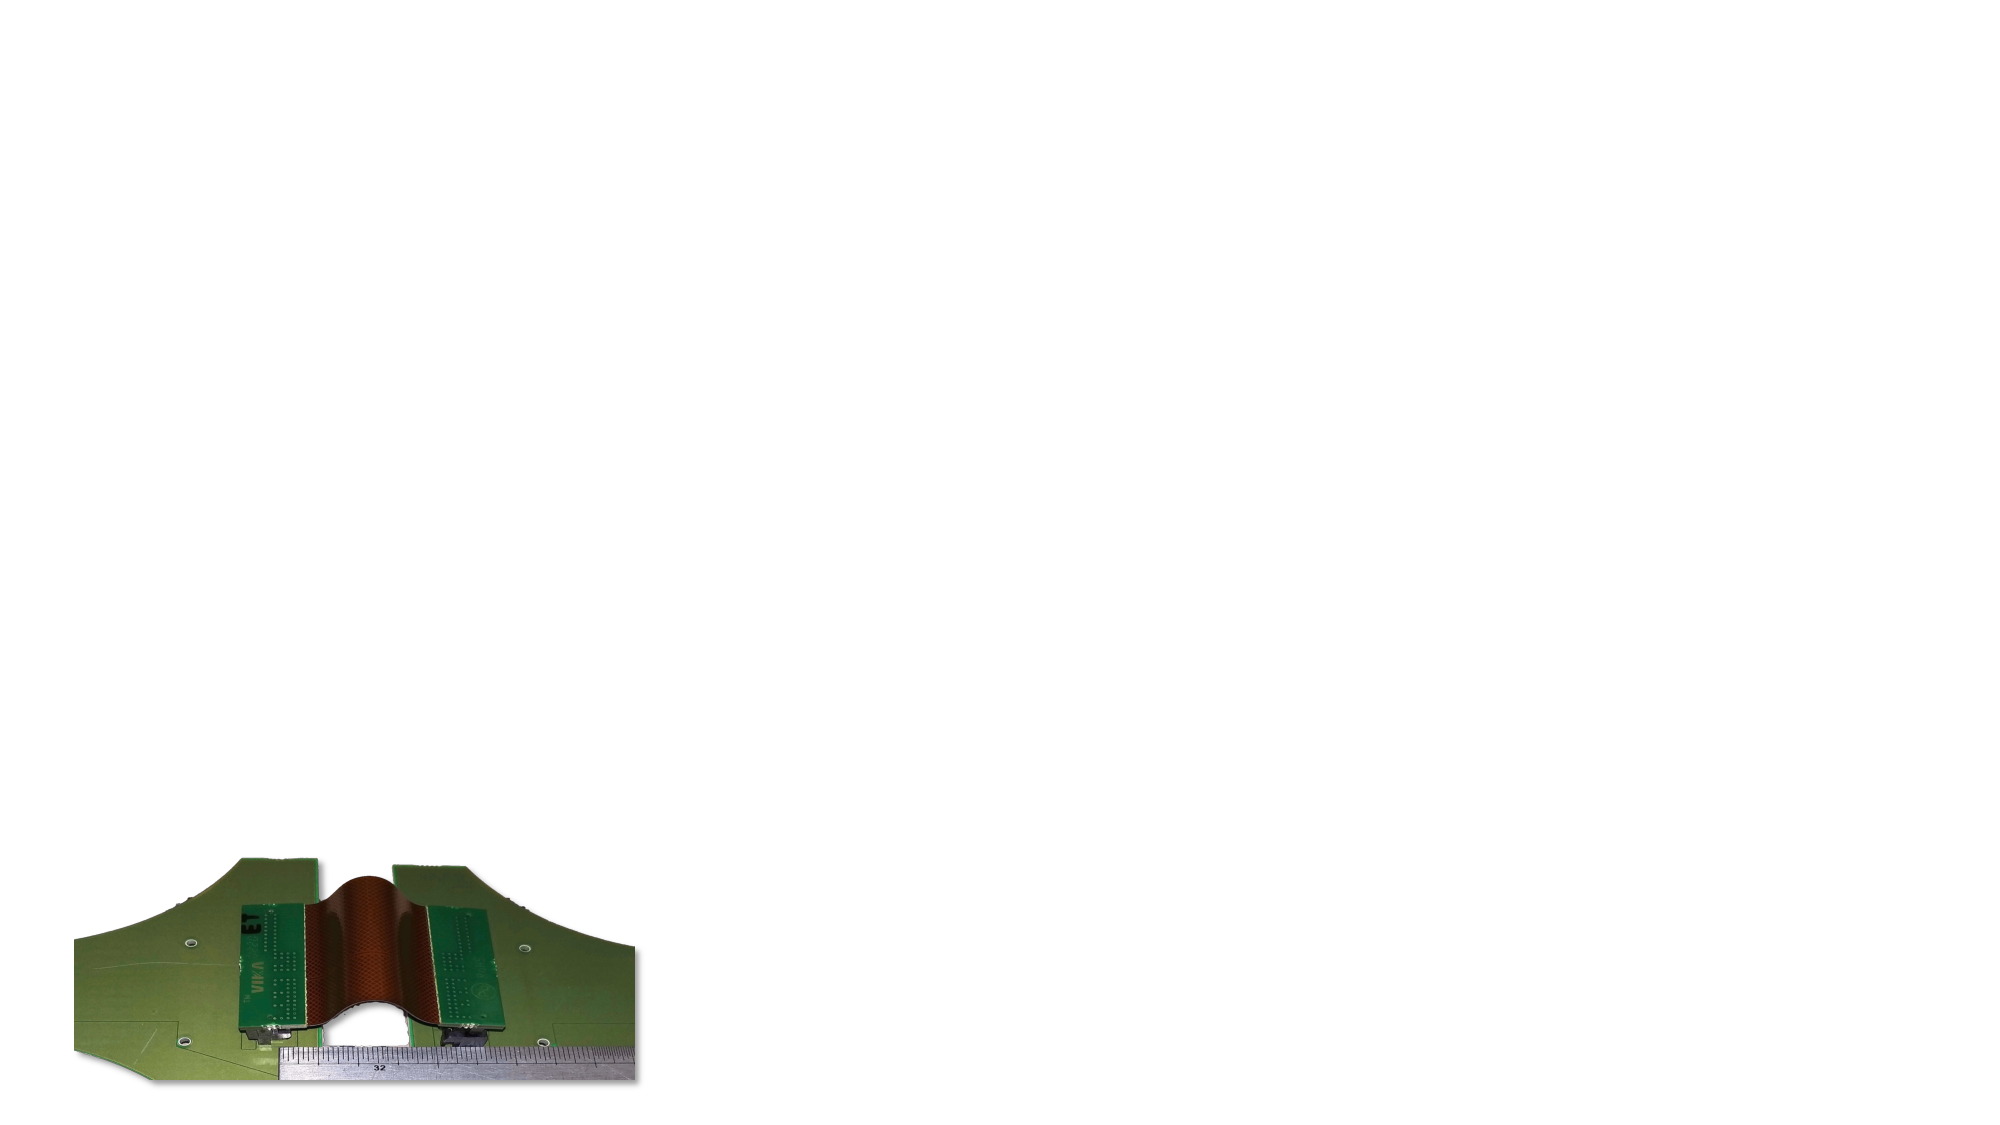
\includegraphics[width=0.475\textwidth]{Images/chap2/flex_rigid_two_FEBs.pdf}\\
    \end{tabular}
    \caption{Flex-rigid board (on the left) connected to two front-end boards in series, where its flexibility can be appreciated.}
    \label{figDflexrigidPIC}
\end{figure}

\par
As done for the front-end boards, a test report has been generated, whose first page is shown in \hyperref[figFLEXreport]{Figure \ref{figFLEXreport}}. In the case of the flex-rigid boards, a single multi-page document has been produced, having the following structure:

\begin{table}[h!]
    \centering
    \def\arraystretch{2}
    \resizebox{0.6\columnwidth}{!}{
        \begin{tabular}{|c|c|c|c|c|} 
            \hline
            $\bm{\#}$ & \textbf{Board ID} & \makecell{\textbf{Thermal}\T \\ \textbf{cycling}\B} & \makecell{\textbf{Visual}\T \\ \textbf{inspection}\B} & \makecell{\textbf{Communication}\T \\ \textbf{test}\B} \\ 
            \hline
            \texttt{1} & \texttt{FR000} & \textcolor{ForestGreen}{\texttt{Yes}}/\textcolor{red}{\texttt{No}} & \textcolor{ForestGreen}{\texttt{Yes}}/\textcolor{red}{\texttt{No}} & \textcolor{ForestGreen}{\texttt{Yes}}/\textcolor{red}{\texttt{No}}\T\B \\ \hline 
        \end{tabular}
    }
    \caption{Structure of the entry for the flex-rigid boards test report.}
    \label{tabFLEXstruct}
\end{table}


%-------------------------------------------------------------------------------
%   Connector for termination
%-------------------------------------------------------------------------------

\section{Connector for termination}

The purpose of the termination connectors is to adapt the \SI{100}{\ohm} differential digital signal tracks through the use of 10 resistors of \SI{100}{\ohm} each soldered onto the connector. The purpose of the tests performed on the termination connectors was to verify the correct installation of the resistors, as well as to ascertain their correct resistance value.

\begin{figure}[ht]
    \centering
    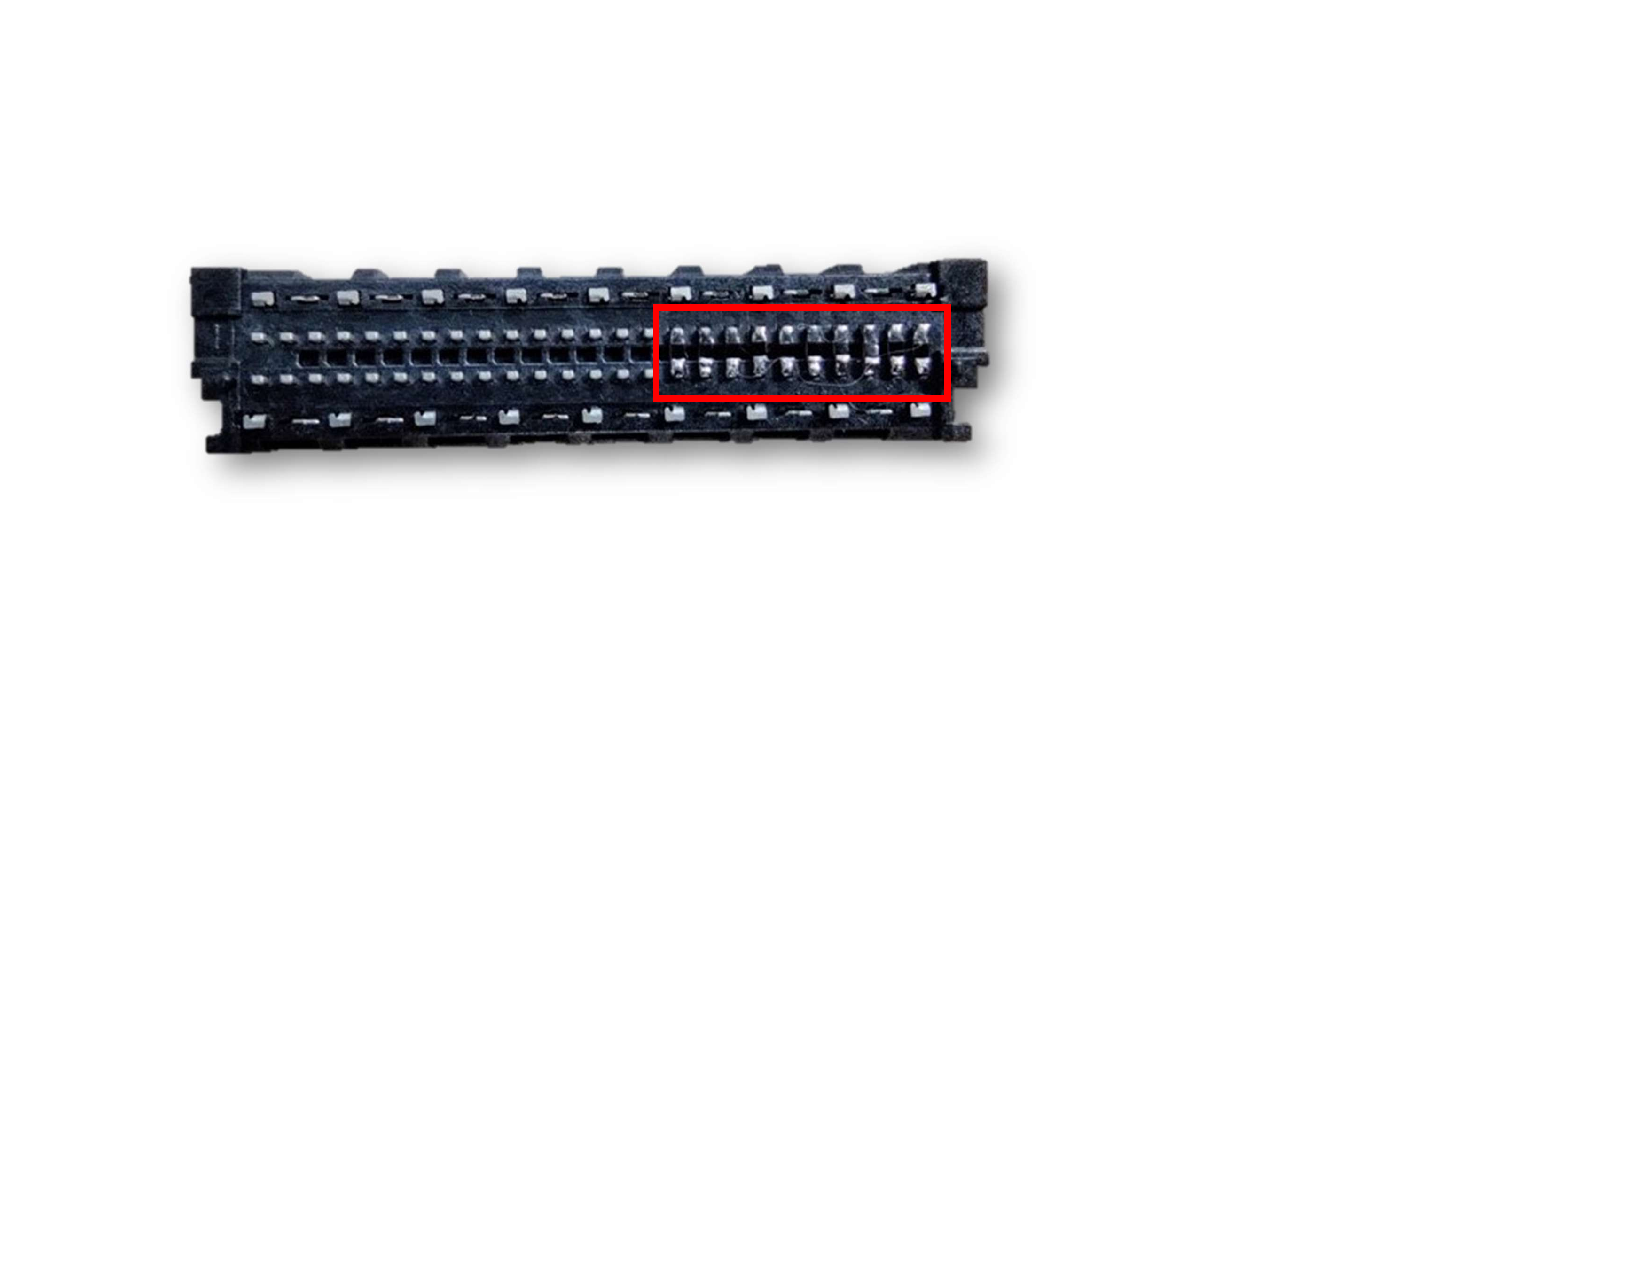
\includegraphics[width=0.45\textwidth]{Images/chap2/term_conn.pdf}
    \caption{Connector for termination with ten \SI{100}{\ohm} resistors installed.}
    \label{figTermConnector}
\end{figure}

\subsection{Visual inspection}
Visual inspection has been carried out to check the connector quality, then look for misaligned pins or missing termination resistor. Visual inspection is carried out before and after the thermal cycle. If no or negligible defects are found, \texttt{[YES]} is reported in the \textit{Visual Inspection} field of the test report.

\subsection{Thermal cycle}
The connectors underwent one thermal cycle in a climate chamber (model ACS DY110). Thermal cycle has the same characteristics described in \hyperref[subsection-thermal]{section \ref{subsection-thermal}}. For connectors that underwent the thermal cycle, \texttt{[YES]} has been reported in the \texttt{Thermal Cycle} field of the test report.

\subsection{Termination resistor soldering}
The quality of the termination resistor soldering has been verified with a digital multimeter by measuring the resistance seen between two pins on the side of the connector opposite with respect to the one where components are mounted. The test has been performed after the thermal cycle for all the 10 termination resistors. If a value of $\approx100\pm\SI{1}{\ohm}$ is found for all the resistors, \texttt{[YES]} is reported in the \textit{Resistor Soldering} field of the test report module.

\par
As done for the front-end boards, a test report has been generated, whose first page is shown in \hyperref[figTERMCONNreport]{Figure \ref{figTERMCONNreport}}. In the case of the connectors for termination, a single multi-page document has been created:

\begin{table}[ht]
    \centering
    \def\arraystretch{1.3}
    \resizebox{0.65\columnwidth}{!}{
        \begin{tabular}{|c|c|c|c|c|} 
            \hline
            $\bm{\#}$ & \textbf{Connector ID} & \makecell{\textbf{Thermal}\T \\ \textbf{cycling}\B} & \makecell{\textbf{Visual}\T \\ \textbf{inspection}\B} & \makecell{\textbf{Resistor}\T \\ \textbf{soldering}\B} \\ 
            \hline
            \texttt{1} & \texttt{T00} & \textcolor{ForestGreen}{\texttt{Yes}}/\textcolor{red}{\texttt{No}} & \textcolor{ForestGreen}{\texttt{Yes}}/\textcolor{red}{\texttt{No}} & \textcolor{ForestGreen}{\texttt{Yes}}/\textcolor{red}{\texttt{No}}\T\B \\ \hline 
        \end{tabular}
    }
    \caption{Structure of the entry for the termination connectors test report.}
    \label{tabTERMCONNstruct}
\end{table}


%-------------------------------------------------------------------------------
%   Front-end board shields
%-------------------------------------------------------------------------------

\section{Front-end board shields} \label{secShield}

The purpose of the front-end board shields, shown in \hyperref[figShieldsAB]{Figure \ref{figShieldsAB}}, is to cover the tracks connecting the Si(Li) sensor strips with the pins of the readout integrated circuit, thereby reducing the impact of electromagnetic induced noise on each of the 32 channels of the readout ASIC.

\subsection{Visual inspection}
Visual inspection has been carried out to check the surface quality, then look for the existence of pits, dents, scratches, pinholes and other defects. Visual inspection was performed before and after the thermal cycle. If no or negligible defects were found, \texttt{[YES]} has been reported in the \textit{Visual Inspection} field of the test report.

\subsection{Thermal cycle}
The boards underwent one thermal cycle in a climate chamber (model ACS DY110). Thermal cycle has the same characteristics described in \hyperref[subsection-thermal]{section \ref{subsection-thermal}}. For the front-end board shields that underwent the thermal cycle, \texttt{[YES]} has been reported in the \textit{Thermal Cycle} field of the test report.

\begin{comment}
    \begin{figure}[h!]
        \centering
        \begin{tabular}{cc}
            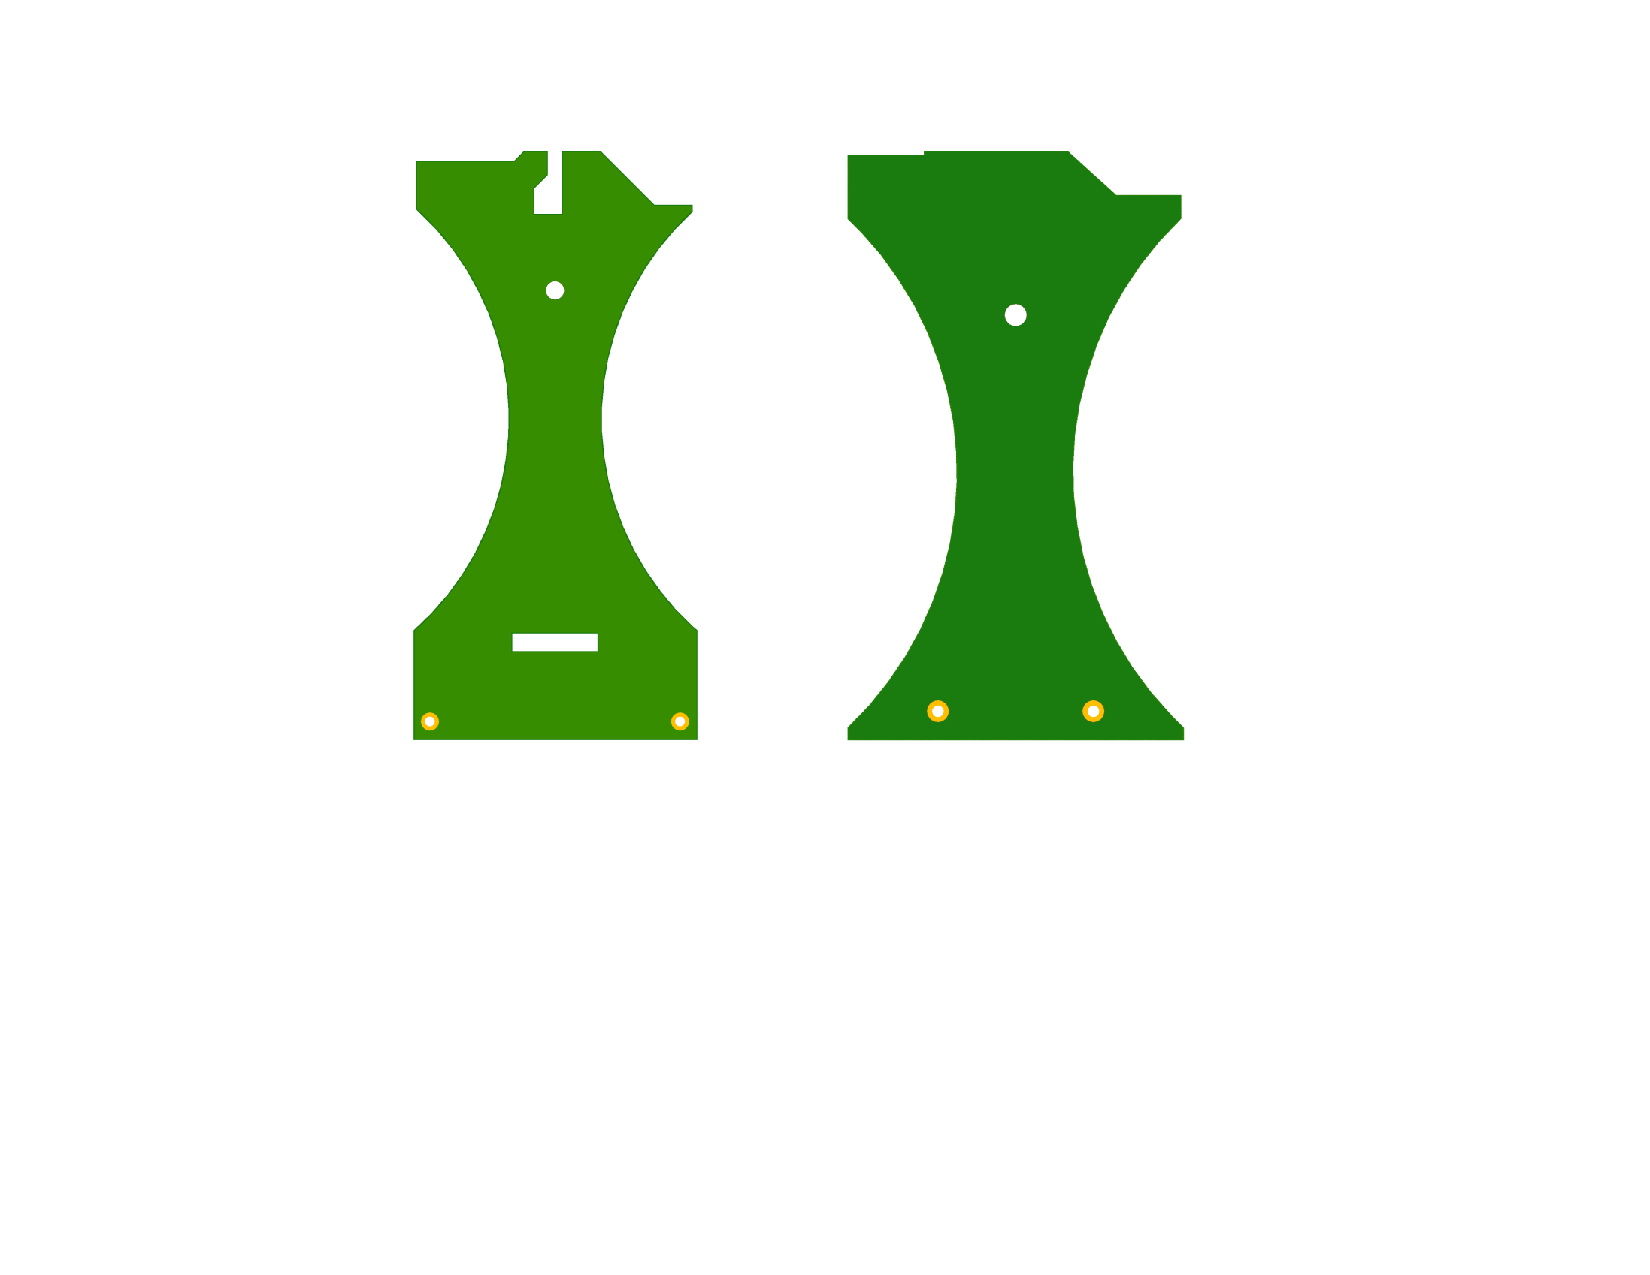
\includegraphics[width=0.5\textwidth]{Images/chap2/shieldsPDFtwo.pdf} & 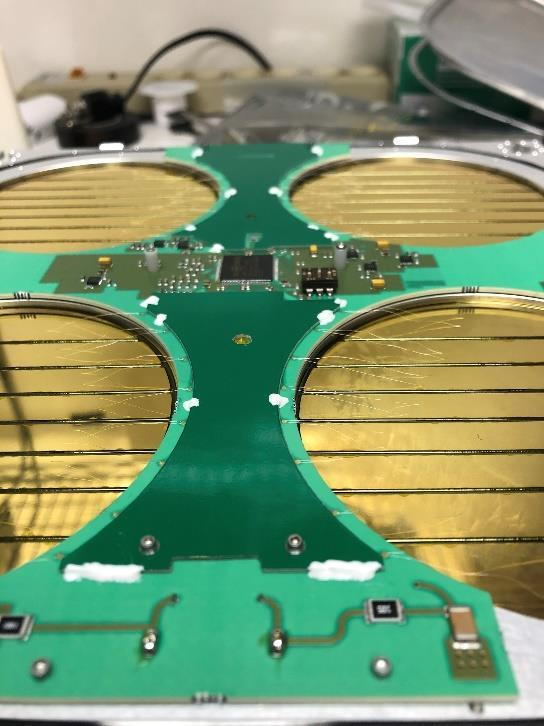
\includegraphics[width=0.3\textwidth]{Images/chap2/Mengjiao_IT_status_PIC.jpg}\\
        \end{tabular}
        \caption{Type A front-end board shield (on the left) and type B front-end board shield (on the right).}
        \label{figShieldsAB}
    \end{figure}
\end{comment}

\begin{figure}[h!]
    \centering
    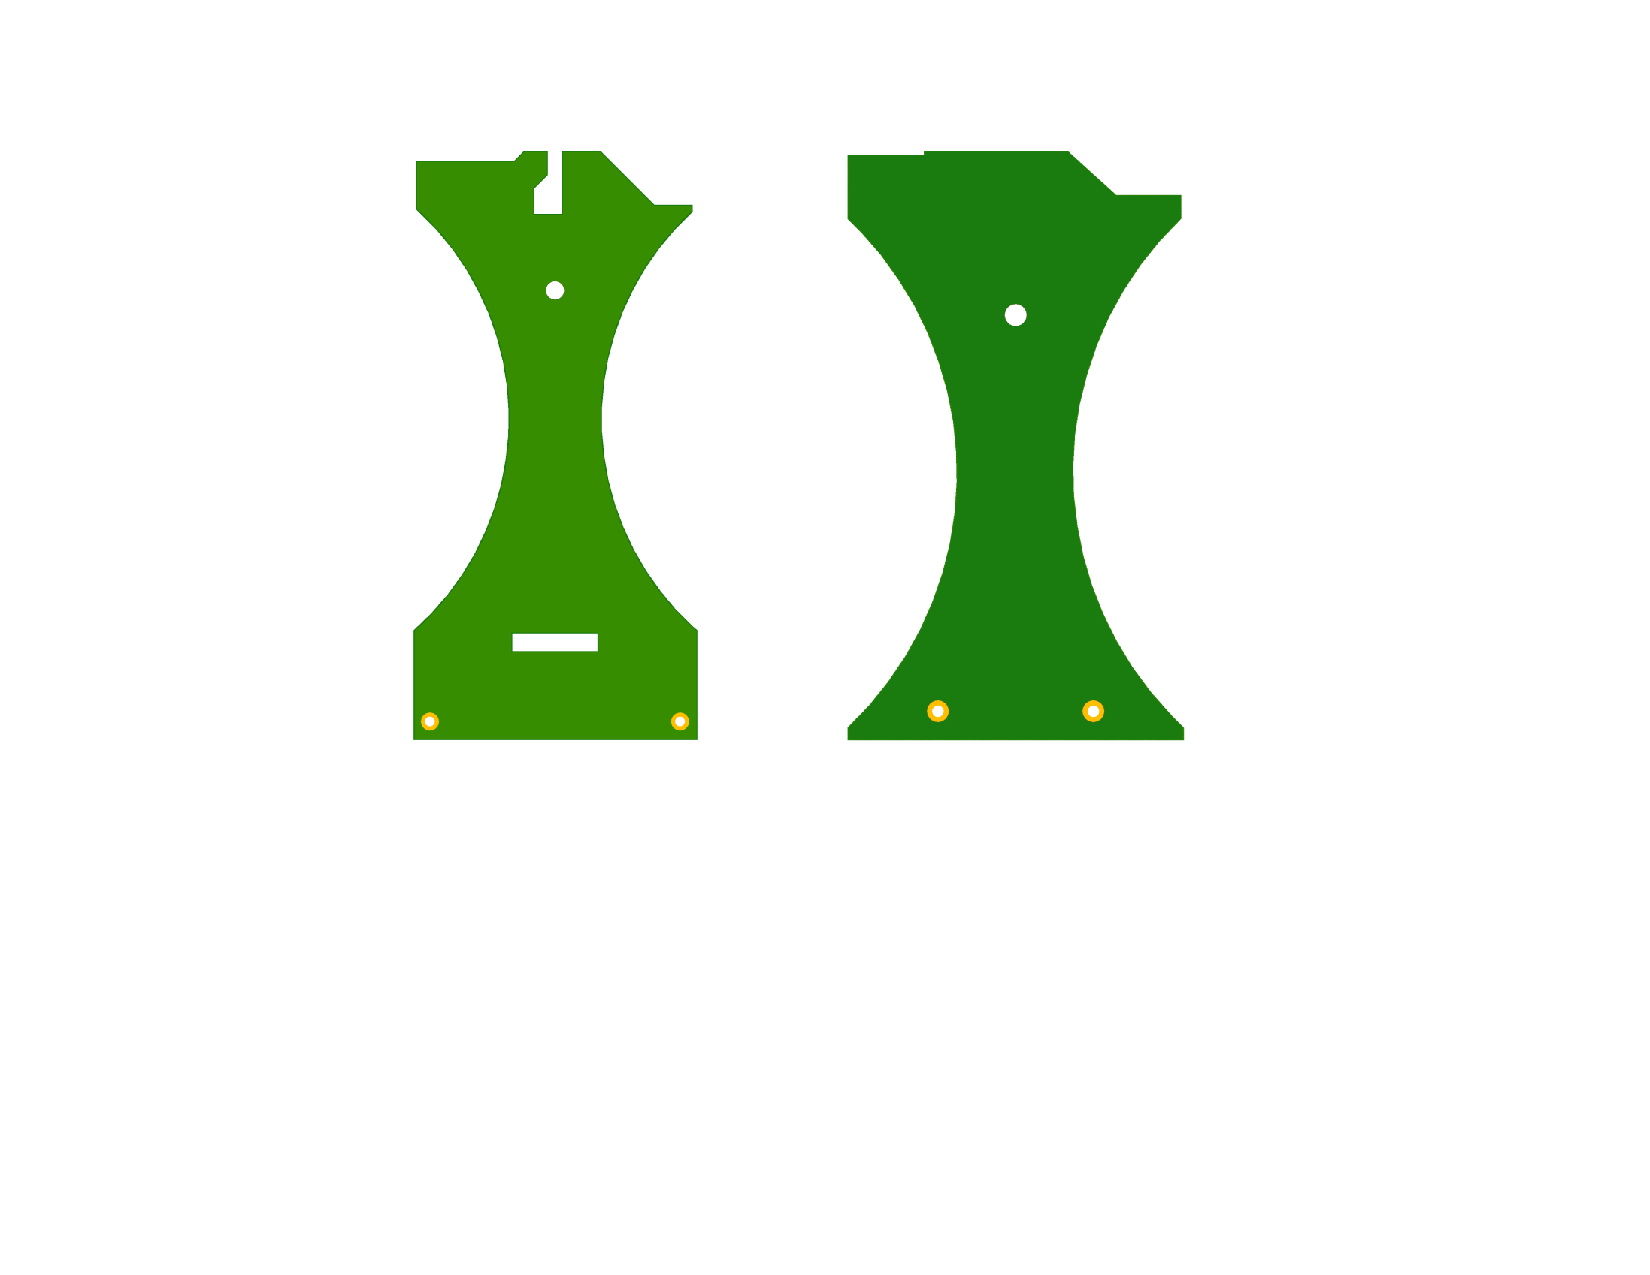
\includegraphics[width=0.6\textwidth]{Images/chap2/shieldsPDFtwo.pdf}
    \caption{Type A front-end board shield (on the left) and type B front-end board shield (on the right).}
    \label{figShieldsAB}
\end{figure}
    

\begin{comment}
    \begin{figure}[h!]
        \centering
        \includegraphics[width=0.5\textwidth]{Images/chap2/FEB_with_shieldsNO.pdf}
        \caption{Type A and type B front-end board shields mounted on a front-end board.}
        \label{figShieldsMounted}
    \end{figure}
\end{comment}

\par
As done for the front-end boards, a test report has been generated, whose first page is shown in \hyperref[figSHIELDreport]{Figure \ref{figSHIELDreport}}. In the case of the front-end board shields, a single multi-page document has been produced, having the structure reported below.

\begin{table}[ht]
    \centering
    \def\arraystretch{1.3}
    \resizebox{0.55\columnwidth}{!}{
        \begin{tabular}{|c|c|c|c|c|} 
            \hline
            $\bm{\#}$ & \textbf{Board ID} & \makecell{\textbf{Thermal}\T \\ \textbf{cycling}\B} & \makecell{\textbf{Visual}\T \\ \textbf{inspection}\B} & \textbf{Note}\T\B \\ 
            \hline
            \texttt{1} & \texttt{FR000} & \textcolor{ForestGreen}{\texttt{Yes}}/\textcolor{red}{\texttt{No}} & \textcolor{ForestGreen}{\texttt{Yes}}/\textcolor{red}{\texttt{No}} & \textit{Note}\T\B \\ \hline 
        \end{tabular}
    }
    \caption{Structure of the entry for the front-end board shields test report.}
    \label{tabSHIELDstruct}
\end{table}
